% Options for packages loaded elsewhere
\PassOptionsToPackage{unicode}{hyperref}
\PassOptionsToPackage{hyphens}{url}
%
\documentclass[
]{article}
\usepackage{amsmath,amssymb}
\usepackage{lmodern}
\usepackage{iftex}
\ifPDFTeX
  \usepackage[T1]{fontenc}
  \usepackage[utf8]{inputenc}
  \usepackage{textcomp} % provide euro and other symbols
\else % if luatex or xetex
  \usepackage{unicode-math}
  \defaultfontfeatures{Scale=MatchLowercase}
  \defaultfontfeatures[\rmfamily]{Ligatures=TeX,Scale=1}
\fi
% Use upquote if available, for straight quotes in verbatim environments
\IfFileExists{upquote.sty}{\usepackage{upquote}}{}
\IfFileExists{microtype.sty}{% use microtype if available
  \usepackage[]{microtype}
  \UseMicrotypeSet[protrusion]{basicmath} % disable protrusion for tt fonts
}{}
\makeatletter
\@ifundefined{KOMAClassName}{% if non-KOMA class
  \IfFileExists{parskip.sty}{%
    \usepackage{parskip}
  }{% else
    \setlength{\parindent}{0pt}
    \setlength{\parskip}{6pt plus 2pt minus 1pt}}
}{% if KOMA class
  \KOMAoptions{parskip=half}}
\makeatother
\usepackage{xcolor}
\usepackage[margin=2.54cm]{geometry}
\usepackage{color}
\usepackage{fancyvrb}
\newcommand{\VerbBar}{|}
\newcommand{\VERB}{\Verb[commandchars=\\\{\}]}
\DefineVerbatimEnvironment{Highlighting}{Verbatim}{commandchars=\\\{\}}
% Add ',fontsize=\small' for more characters per line
\usepackage{framed}
\definecolor{shadecolor}{RGB}{248,248,248}
\newenvironment{Shaded}{\begin{snugshade}}{\end{snugshade}}
\newcommand{\AlertTok}[1]{\textcolor[rgb]{0.94,0.16,0.16}{#1}}
\newcommand{\AnnotationTok}[1]{\textcolor[rgb]{0.56,0.35,0.01}{\textbf{\textit{#1}}}}
\newcommand{\AttributeTok}[1]{\textcolor[rgb]{0.77,0.63,0.00}{#1}}
\newcommand{\BaseNTok}[1]{\textcolor[rgb]{0.00,0.00,0.81}{#1}}
\newcommand{\BuiltInTok}[1]{#1}
\newcommand{\CharTok}[1]{\textcolor[rgb]{0.31,0.60,0.02}{#1}}
\newcommand{\CommentTok}[1]{\textcolor[rgb]{0.56,0.35,0.01}{\textit{#1}}}
\newcommand{\CommentVarTok}[1]{\textcolor[rgb]{0.56,0.35,0.01}{\textbf{\textit{#1}}}}
\newcommand{\ConstantTok}[1]{\textcolor[rgb]{0.00,0.00,0.00}{#1}}
\newcommand{\ControlFlowTok}[1]{\textcolor[rgb]{0.13,0.29,0.53}{\textbf{#1}}}
\newcommand{\DataTypeTok}[1]{\textcolor[rgb]{0.13,0.29,0.53}{#1}}
\newcommand{\DecValTok}[1]{\textcolor[rgb]{0.00,0.00,0.81}{#1}}
\newcommand{\DocumentationTok}[1]{\textcolor[rgb]{0.56,0.35,0.01}{\textbf{\textit{#1}}}}
\newcommand{\ErrorTok}[1]{\textcolor[rgb]{0.64,0.00,0.00}{\textbf{#1}}}
\newcommand{\ExtensionTok}[1]{#1}
\newcommand{\FloatTok}[1]{\textcolor[rgb]{0.00,0.00,0.81}{#1}}
\newcommand{\FunctionTok}[1]{\textcolor[rgb]{0.00,0.00,0.00}{#1}}
\newcommand{\ImportTok}[1]{#1}
\newcommand{\InformationTok}[1]{\textcolor[rgb]{0.56,0.35,0.01}{\textbf{\textit{#1}}}}
\newcommand{\KeywordTok}[1]{\textcolor[rgb]{0.13,0.29,0.53}{\textbf{#1}}}
\newcommand{\NormalTok}[1]{#1}
\newcommand{\OperatorTok}[1]{\textcolor[rgb]{0.81,0.36,0.00}{\textbf{#1}}}
\newcommand{\OtherTok}[1]{\textcolor[rgb]{0.56,0.35,0.01}{#1}}
\newcommand{\PreprocessorTok}[1]{\textcolor[rgb]{0.56,0.35,0.01}{\textit{#1}}}
\newcommand{\RegionMarkerTok}[1]{#1}
\newcommand{\SpecialCharTok}[1]{\textcolor[rgb]{0.00,0.00,0.00}{#1}}
\newcommand{\SpecialStringTok}[1]{\textcolor[rgb]{0.31,0.60,0.02}{#1}}
\newcommand{\StringTok}[1]{\textcolor[rgb]{0.31,0.60,0.02}{#1}}
\newcommand{\VariableTok}[1]{\textcolor[rgb]{0.00,0.00,0.00}{#1}}
\newcommand{\VerbatimStringTok}[1]{\textcolor[rgb]{0.31,0.60,0.02}{#1}}
\newcommand{\WarningTok}[1]{\textcolor[rgb]{0.56,0.35,0.01}{\textbf{\textit{#1}}}}
\usepackage{graphicx}
\makeatletter
\def\maxwidth{\ifdim\Gin@nat@width>\linewidth\linewidth\else\Gin@nat@width\fi}
\def\maxheight{\ifdim\Gin@nat@height>\textheight\textheight\else\Gin@nat@height\fi}
\makeatother
% Scale images if necessary, so that they will not overflow the page
% margins by default, and it is still possible to overwrite the defaults
% using explicit options in \includegraphics[width, height, ...]{}
\setkeys{Gin}{width=\maxwidth,height=\maxheight,keepaspectratio}
% Set default figure placement to htbp
\makeatletter
\def\fps@figure{htbp}
\makeatother
\setlength{\emergencystretch}{3em} % prevent overfull lines
\providecommand{\tightlist}{%
  \setlength{\itemsep}{0pt}\setlength{\parskip}{0pt}}
\setcounter{secnumdepth}{-\maxdimen} % remove section numbering
\usepackage{booktabs}
\usepackage{longtable}
\usepackage{array}
\usepackage{multirow}
\usepackage{wrapfig}
\usepackage{float}
\usepackage{colortbl}
\usepackage{pdflscape}
\usepackage{tabu}
\usepackage{threeparttable}
\usepackage{threeparttablex}
\usepackage[normalem]{ulem}
\usepackage{makecell}
\usepackage{xcolor}
\ifLuaTeX
  \usepackage{selnolig}  % disable illegal ligatures
\fi
\IfFileExists{bookmark.sty}{\usepackage{bookmark}}{\usepackage{hyperref}}
\IfFileExists{xurl.sty}{\usepackage{xurl}}{} % add URL line breaks if available
\urlstyle{same} % disable monospaced font for URLs
\hypersetup{
  pdftitle={Visionary Final},
  pdfauthor={Justin DePue, John Rooney, and Tony Jiang},
  hidelinks,
  pdfcreator={LaTeX via pandoc}}

\title{Visionary Final}
\author{Justin DePue, John Rooney, and Tony Jiang}
\date{2023-04-26}

\begin{document}
\maketitle

\hypertarget{library-packages}{%
\subsection{library packages}\label{library-packages}}

\begin{Shaded}
\begin{Highlighting}[]
\FunctionTok{library}\NormalTok{(tseries)}
\FunctionTok{library}\NormalTok{(lubridate)}
\FunctionTok{library}\NormalTok{(here)}
\FunctionTok{library}\NormalTok{(tidyverse)}
\FunctionTok{library}\NormalTok{(outliers)}
\FunctionTok{library}\NormalTok{(ggplot2)}
\FunctionTok{library}\NormalTok{(forecast)}
\FunctionTok{library}\NormalTok{(kableExtra)}
\FunctionTok{library}\NormalTok{(readxl)}
\end{Highlighting}
\end{Shaded}

\hypertarget{load-the-data}{%
\subsection{load the data}\label{load-the-data}}

\begin{Shaded}
\begin{Highlighting}[]
\CommentTok{\# automatically set the working directory as personal local path to R project}
\CommentTok{\# so the file path in read.csv can work for everyone}
\FunctionTok{setwd}\NormalTok{(}\FunctionTok{here}\NormalTok{())}

\CommentTok{\# load the data}
\NormalTok{electricity\_prices.df }\OtherTok{\textless{}{-}} \FunctionTok{read.csv}\NormalTok{(}\StringTok{"./Data/Average\_retail\_price\_of\_electricity.csv"}\NormalTok{, }\AttributeTok{header =} \ConstantTok{TRUE}\NormalTok{, }\AttributeTok{skip=}\DecValTok{4}\NormalTok{)}

\NormalTok{nc\_electricity.df}\OtherTok{\textless{}{-}}\NormalTok{electricity\_prices.df[}\DecValTok{228}\NormalTok{,}\DecValTok{4}\SpecialCharTok{:}\NormalTok{(}\FunctionTok{ncol}\NormalTok{(electricity\_prices.df))] }\SpecialCharTok{\%\textgreater{}\%}
  \FunctionTok{pivot\_longer}\NormalTok{(}\AttributeTok{cols=}\FunctionTok{everything}\NormalTok{(), }\AttributeTok{names\_to =} \StringTok{\textquotesingle{}my\_date\textquotesingle{}}\NormalTok{, }\AttributeTok{values\_to =} \StringTok{\textquotesingle{}price\_per\_kWh\textquotesingle{}}\NormalTok{)}

\CommentTok{\# examine whether there is missing value or not}
\FunctionTok{summary}\NormalTok{(nc\_electricity.df)}
\end{Highlighting}
\end{Shaded}

\begin{verbatim}
##    my_date          price_per_kWh     
##  Length:265         Length:265        
##  Class :character   Class :character  
##  Mode  :character   Mode  :character
\end{verbatim}

\begin{Shaded}
\begin{Highlighting}[]
\CommentTok{\# there is no missing value}

\NormalTok{nc\_electricity.df}\SpecialCharTok{$}\NormalTok{price\_per\_kWh}\OtherTok{\textless{}{-}}\FunctionTok{as.numeric}\NormalTok{(nc\_electricity.df}\SpecialCharTok{$}\NormalTok{price\_per\_kWh)}
  

\CommentTok{\# Import Natural Gas data}

\NormalTok{natural\_gas.df }\OtherTok{\textless{}{-}} \FunctionTok{read.csv}\NormalTok{(}\StringTok{"./Data/NC\_NaturalGas.csv"}\NormalTok{, }\AttributeTok{header =} \ConstantTok{TRUE}\NormalTok{, }\AttributeTok{skip=}\DecValTok{2}\NormalTok{,}\AttributeTok{col.names =} \FunctionTok{c}\NormalTok{(}\StringTok{"year"}\NormalTok{, }\StringTok{"price"}\NormalTok{))}

\CommentTok{\#Check for missing data. There is an extra row with an NA at the end of the data, so I removed it with na.omit}

\FunctionTok{summary}\NormalTok{(}\FunctionTok{na.omit}\NormalTok{(natural\_gas.df))}
\end{Highlighting}
\end{Shaded}

\begin{verbatim}
##      year               price      
##  Length:409         Min.   : 5.54  
##  Class :character   1st Qu.: 9.07  
##  Mode  :character   Median :12.54  
##                     Mean   :13.78  
##                     3rd Qu.:18.11  
##                     Max.   :30.43
\end{verbatim}

\begin{Shaded}
\begin{Highlighting}[]
\FunctionTok{str}\NormalTok{(natural\_gas.df)}
\end{Highlighting}
\end{Shaded}

\begin{verbatim}
## 'data.frame':    410 obs. of  2 variables:
##  $ year : chr  "Jan-1989" "Feb-1989" "Mar-1989" "Apr-1989" ...
##  $ price: num  6.17 6.3 6.29 6.8 6.99 8.02 8.71 8.97 8.68 7.44 ...
\end{verbatim}

\begin{Shaded}
\begin{Highlighting}[]
\CommentTok{\#create timeseries for natural gas}

\NormalTok{ts\_NG}\OtherTok{\textless{}{-}}\FunctionTok{ts}\NormalTok{(}\FunctionTok{na.omit}\NormalTok{(natural\_gas.df[,}\DecValTok{2}\NormalTok{]), }\AttributeTok{start=}\FunctionTok{c}\NormalTok{(}\DecValTok{1989}\NormalTok{,}\DecValTok{1}\NormalTok{), }\AttributeTok{frequency=}\DecValTok{12}\NormalTok{)}

\CommentTok{\# plot raw time series}
\FunctionTok{plot}\NormalTok{(ts\_NG, }\AttributeTok{col=}\StringTok{"blue"}\NormalTok{, }\AttributeTok{ylab=}\StringTok{"$/Mcf"}\NormalTok{, }\AttributeTok{xlab=}\StringTok{"Date"}\NormalTok{, }\AttributeTok{main=}\StringTok{"NC Residential Natural Gas Cost"}\NormalTok{)}
\end{Highlighting}
\end{Shaded}

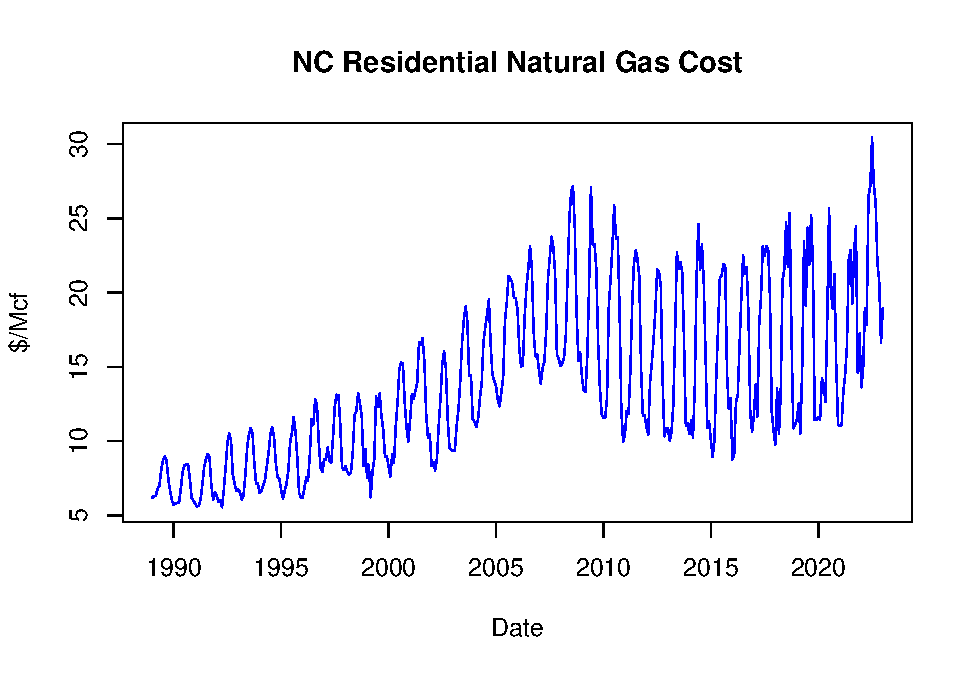
\includegraphics{Final-Project_files/figure-latex/unnamed-chunk-2-1.pdf}

\hypertarget{standardize-the-unit-of-natural-gas-data-to-make-it-comparable-with-electricity}{%
\subsection{standardize the unit of natural gas data to make it
comparable with
electricity}\label{standardize-the-unit-of-natural-gas-data-to-make-it-comparable-with-electricity}}

\begin{Shaded}
\begin{Highlighting}[]
\CommentTok{\# convert natural gas data from $/Mcf to $/kWh based on 80\% heating efficiency}
\CommentTok{\# $/kWh = [($/mcf/1.037)/293.07107]/0.9 = $/mcf/273.52}


\NormalTok{conversion }\OtherTok{\textless{}{-}} \FloatTok{0.8}\SpecialCharTok{*}\FloatTok{293.07107}\SpecialCharTok{*}\FloatTok{1.037}\SpecialCharTok{/}\DecValTok{100}


\NormalTok{natural\_gas.df}\SpecialCharTok{$}\NormalTok{kwh\_equiv}\OtherTok{\textless{}{-}}\NormalTok{((natural\_gas.df}\SpecialCharTok{$}\NormalTok{price)}\SpecialCharTok{/}\NormalTok{conversion)}


\NormalTok{natural\_gas.df}\OtherTok{\textless{}{-}}\FunctionTok{na.omit}\NormalTok{(natural\_gas.df)}

\NormalTok{ts\_gas\_equiv}\OtherTok{\textless{}{-}}\FunctionTok{ts}\NormalTok{(natural\_gas.df[,}\DecValTok{3}\NormalTok{], }\AttributeTok{start=}\FunctionTok{c}\NormalTok{(}\DecValTok{1989}\NormalTok{,}\DecValTok{1}\NormalTok{), }\AttributeTok{frequency=}\DecValTok{12}\NormalTok{)}

\NormalTok{ts\_gas\_equiv}\OtherTok{\textless{}{-}}\FunctionTok{window}\NormalTok{(ts\_gas\_equiv, }\AttributeTok{start=}\FunctionTok{c}\NormalTok{(}\DecValTok{2001}\NormalTok{, }\DecValTok{1}\NormalTok{))}

\CommentTok{\#plot gas TS in kw/hr equiv}
\FunctionTok{autoplot}\NormalTok{(ts\_gas\_equiv) }\SpecialCharTok{+}
  \FunctionTok{ylab}\NormalTok{(}\StringTok{"Price (cents/kWh"}\NormalTok{) }\SpecialCharTok{+} 
  \FunctionTok{ggtitle}\NormalTok{(}\StringTok{"Natural Gas Price (cents/kWh)"}\NormalTok{)}
\end{Highlighting}
\end{Shaded}

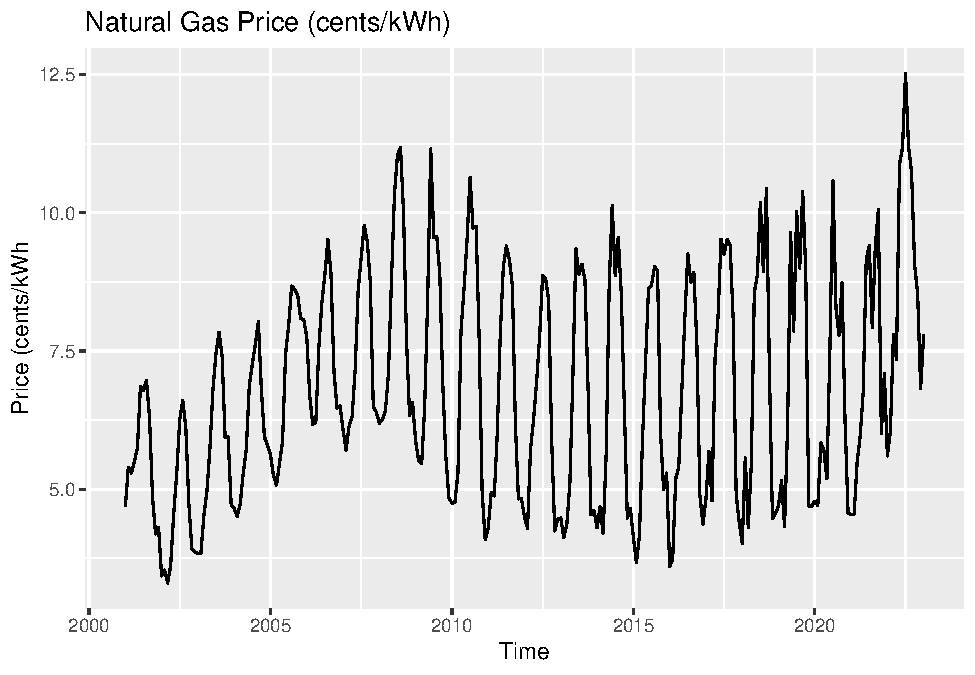
\includegraphics{Final-Project_files/figure-latex/unnamed-chunk-3-1.pdf}

\begin{Shaded}
\begin{Highlighting}[]
\CommentTok{\# coerce electricity to a time series object}

\NormalTok{ts\_electricity}\OtherTok{\textless{}{-}}\FunctionTok{ts}\NormalTok{(}\FunctionTok{rev}\NormalTok{(nc\_electricity.df[,}\DecValTok{2}\NormalTok{]), }\AttributeTok{start=}\FunctionTok{c}\NormalTok{(}\DecValTok{2001}\NormalTok{,}\DecValTok{1}\NormalTok{), }\AttributeTok{frequency=}\DecValTok{12}\NormalTok{)}

\FunctionTok{plot}\NormalTok{(ts\_electricity, }\AttributeTok{col=}\StringTok{"red"}\NormalTok{, }\AttributeTok{ylab=}\StringTok{"$/kWh"}\NormalTok{, }\AttributeTok{xlab=}\StringTok{"Date"}\NormalTok{, }\AttributeTok{main=}\StringTok{"NC Residential Electricity Cost"}\NormalTok{)}
\end{Highlighting}
\end{Shaded}

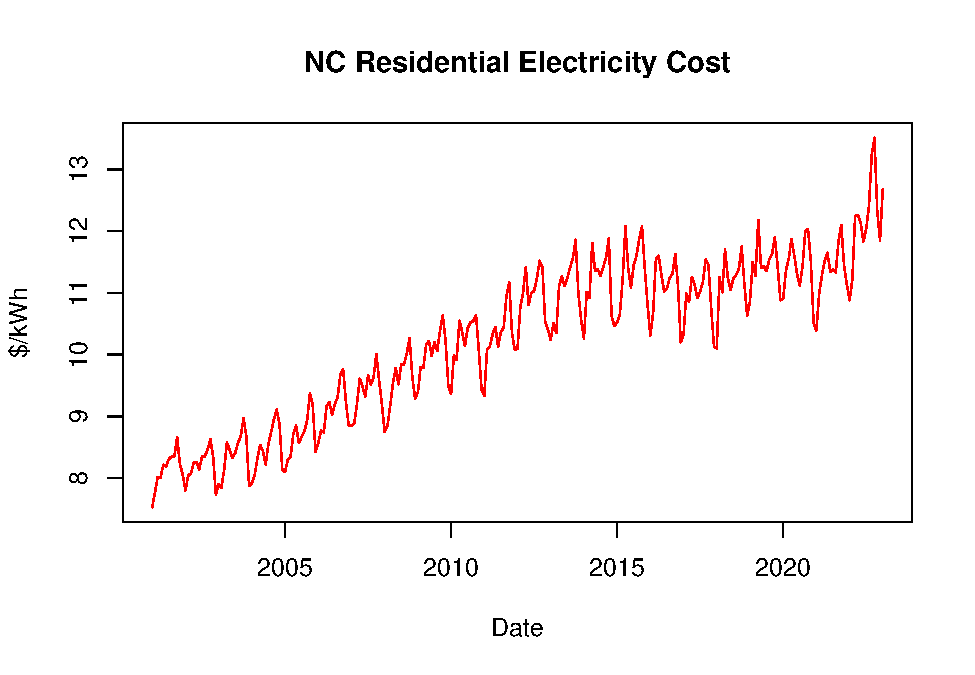
\includegraphics{Final-Project_files/figure-latex/unnamed-chunk-3-2.pdf}

\begin{Shaded}
\begin{Highlighting}[]
\CommentTok{\#plot both electric \& gas TS together}
\FunctionTok{ts.plot}\NormalTok{(ts\_gas\_equiv, ts\_electricity, }\AttributeTok{gpars =} \FunctionTok{list}\NormalTok{(}\AttributeTok{col =} \FunctionTok{c}\NormalTok{(}\StringTok{"red"}\NormalTok{, }\StringTok{"blue"}\NormalTok{)), }
        \AttributeTok{xlab=}\StringTok{"Date"}\NormalTok{, }\AttributeTok{ylab=}\StringTok{"cents/kWh"}\NormalTok{, }
        \AttributeTok{main=}\StringTok{"Comparison of Natural Gas and Electricity Costs"}\NormalTok{)}
\FunctionTok{legend}\NormalTok{(}\StringTok{"topleft"}\NormalTok{, }\AttributeTok{bty=}\StringTok{"n"}\NormalTok{, }\AttributeTok{lty=}\FunctionTok{c}\NormalTok{(}\DecValTok{1}\NormalTok{,}\DecValTok{1}\NormalTok{), }\AttributeTok{col=}\FunctionTok{c}\NormalTok{(}\StringTok{"red"}\NormalTok{,}\StringTok{"blue"}\NormalTok{),}
       \AttributeTok{legend=}\FunctionTok{c}\NormalTok{(}\StringTok{" Natural Gas "}\NormalTok{, }\StringTok{" Electricity "}\NormalTok{))}
\end{Highlighting}
\end{Shaded}

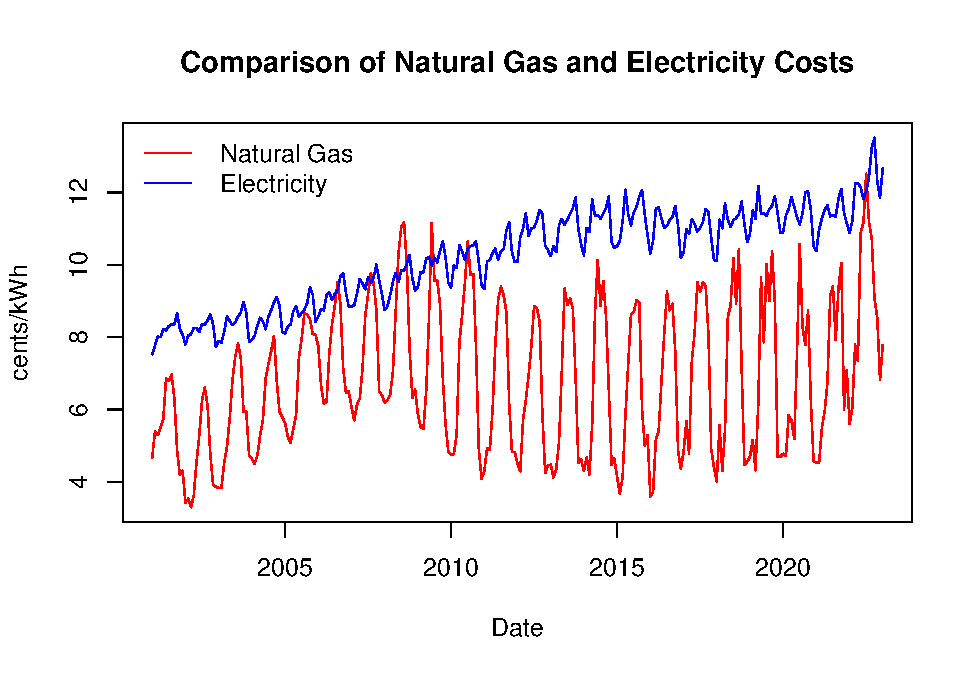
\includegraphics{Final-Project_files/figure-latex/unnamed-chunk-3-3.pdf}

\begin{Shaded}
\begin{Highlighting}[]
\CommentTok{\#Create Dataframe with both Gas \& Electricity prices...}
\CommentTok{\#create new date column}
\NormalTok{new\_date}\OtherTok{\textless{}{-}}\FunctionTok{seq}\NormalTok{(}\FunctionTok{as.Date}\NormalTok{(}\StringTok{"2001/1/1"}\NormalTok{), }\AttributeTok{by =} \StringTok{"month"}\NormalTok{, }\AttributeTok{length.out =} \FunctionTok{nrow}\NormalTok{(ts\_electricity))}

\CommentTok{\#bind date, gas, \& electricity}
\NormalTok{nc\_energy.df}\OtherTok{\textless{}{-}}\FunctionTok{cbind.data.frame}\NormalTok{(}\StringTok{"Month\_Date"}\OtherTok{=}\NormalTok{new\_date, }
                               \StringTok{"electricity"}\OtherTok{=}\NormalTok{nc\_electricity.df}\SpecialCharTok{$}\NormalTok{price\_per\_kWh, }
                               \StringTok{"gas\_equiv"}\OtherTok{=}\NormalTok{ts\_gas\_equiv)}

\CommentTok{\#Subtract Gas price from Electricity price}
\NormalTok{nc\_energy.df}\SpecialCharTok{$}\NormalTok{cost\_diff}\OtherTok{\textless{}{-}}\NormalTok{(nc\_energy.df}\SpecialCharTok{$}\NormalTok{electricity }\SpecialCharTok{{-}}\NormalTok{ nc\_energy.df}\SpecialCharTok{$}\NormalTok{gas\_equiv)}
\end{Highlighting}
\end{Shaded}

\hypertarget{add-covariates}{%
\subsection{add covariates}\label{add-covariates}}

\begin{Shaded}
\begin{Highlighting}[]
\CommentTok{\# create an indicator variable for Ukraine War for gas}

\CommentTok{\# create a column with row index}
\NormalTok{natural\_gas.df }\OtherTok{\textless{}{-}} \FunctionTok{rownames\_to\_column}\NormalTok{(natural\_gas.df, }\AttributeTok{var =} \StringTok{"index"}\NormalTok{)}

\NormalTok{natural\_gas.df}\SpecialCharTok{$}\NormalTok{index }\OtherTok{=} \FunctionTok{as.numeric}\NormalTok{(natural\_gas.df}\SpecialCharTok{$}\NormalTok{index)}

\NormalTok{natural\_gas.df}\SpecialCharTok{$}\NormalTok{UKRWAR }\OtherTok{\textless{}{-}} \FunctionTok{ifelse}\NormalTok{(natural\_gas.df}\SpecialCharTok{$}\NormalTok{index }\SpecialCharTok{\textgreater{}=} \DecValTok{399}\NormalTok{, }\DecValTok{1}\NormalTok{, }\DecValTok{0}\NormalTok{)}

\NormalTok{natural\_gas.df }\OtherTok{\textless{}{-}}\NormalTok{ natural\_gas.df[, }\FunctionTok{c}\NormalTok{(}\SpecialCharTok{{-}}\DecValTok{1}\NormalTok{, }\SpecialCharTok{{-}}\DecValTok{6}\NormalTok{)]}

\NormalTok{ts\_gas\_equiv}\OtherTok{\textless{}{-}}\FunctionTok{ts}\NormalTok{(natural\_gas.df[,}\FunctionTok{c}\NormalTok{(}\DecValTok{3}\NormalTok{,}\DecValTok{4}\NormalTok{)], }\AttributeTok{start=}\FunctionTok{c}\NormalTok{(}\DecValTok{1989}\NormalTok{,}\DecValTok{1}\NormalTok{), }\AttributeTok{frequency=}\DecValTok{12}\NormalTok{) }\SpecialCharTok{\%\textgreater{}\%} 
  \FunctionTok{window}\NormalTok{(}\AttributeTok{start =} \FunctionTok{c}\NormalTok{(}\DecValTok{2001}\NormalTok{, }\DecValTok{1}\NormalTok{))}

\CommentTok{\# create an indicator variable for Ukraine War for electricity}
\NormalTok{nc\_electricity.df }\OtherTok{\textless{}{-}} \FunctionTok{rownames\_to\_column}\NormalTok{(nc\_electricity.df, }\AttributeTok{var =} \StringTok{"index"}\NormalTok{)}

\NormalTok{nc\_electricity.df}\SpecialCharTok{$}\NormalTok{index }\OtherTok{\textless{}{-}} \FunctionTok{as.numeric}\NormalTok{(nc\_electricity.df}\SpecialCharTok{$}\NormalTok{index)}

\NormalTok{nc\_electricity.df}\SpecialCharTok{$}\NormalTok{UKRWAR }\OtherTok{\textless{}{-}} \FunctionTok{ifelse}\NormalTok{(nc\_electricity.df}\SpecialCharTok{$}\NormalTok{index }\SpecialCharTok{\textgreater{}=} \DecValTok{255}\NormalTok{, }\DecValTok{1}\NormalTok{, }\DecValTok{0}\NormalTok{)}

\NormalTok{nc\_electricity.df }\OtherTok{\textless{}{-}}\NormalTok{ nc\_electricity.df[, }\SpecialCharTok{{-}}\DecValTok{1}\NormalTok{]}

\CommentTok{\# coerce electricity to a time series object}

\NormalTok{ts\_electricity}\OtherTok{\textless{}{-}}\FunctionTok{ts}\NormalTok{(}\FunctionTok{rev}\NormalTok{(nc\_electricity.df[,}\DecValTok{2}\SpecialCharTok{:}\DecValTok{3}\NormalTok{]), }\AttributeTok{start=}\FunctionTok{c}\NormalTok{(}\DecValTok{2001}\NormalTok{,}\DecValTok{1}\NormalTok{), }\AttributeTok{frequency=}\DecValTok{12}\NormalTok{)}


\CommentTok{\# import temperature data}
\NormalTok{temperautre }\OtherTok{\textless{}{-}} \FunctionTok{read\_xlsx}\NormalTok{(}\StringTok{"./Data/Raleigh Temperature.xlsx"}\NormalTok{) }\SpecialCharTok{\%\textgreater{}\%} 
  \FunctionTok{gather}\NormalTok{(}\AttributeTok{key =} \StringTok{"Month"}\NormalTok{, }\AttributeTok{value =} \StringTok{"temperature"}\NormalTok{, Jan, Feb, Mar, Apr, May, Jun, Jul, Aug, Sep, Oct, Nov, Dec)}

\NormalTok{temperautre }\OtherTok{\textless{}{-}}\NormalTok{ temperautre[}\FunctionTok{order}\NormalTok{(temperautre}\SpecialCharTok{$}\NormalTok{Year), ] }

\NormalTok{ts\_temperature }\OtherTok{\textless{}{-}}\NormalTok{ temperautre[,}\DecValTok{3}\NormalTok{] }\SpecialCharTok{\%\textgreater{}\%} 
  \FunctionTok{na.omit}\NormalTok{() }\SpecialCharTok{\%\textgreater{}\%} 
  \FunctionTok{ts}\NormalTok{(}\AttributeTok{start =} \FunctionTok{c}\NormalTok{(}\DecValTok{1995}\NormalTok{, }\DecValTok{1}\NormalTok{), }\AttributeTok{frequency =} \DecValTok{12}\NormalTok{) }\SpecialCharTok{\%\textgreater{}\%} 
  \FunctionTok{window}\NormalTok{(}\AttributeTok{start =} \FunctionTok{c}\NormalTok{(}\DecValTok{2001}\NormalTok{, }\DecValTok{1}\NormalTok{), }\AttributeTok{end =} \FunctionTok{c}\NormalTok{(}\DecValTok{2023}\NormalTok{, }\DecValTok{1}\NormalTok{))}

\CommentTok{\# create a data frame for covariates for electricity (2001{-}2022)}
\CommentTok{\# we need to do this because electricity and natural gas }
\CommentTok{\# have different fourier terms}
\NormalTok{fourier\_train\_e }\OtherTok{\textless{}{-}} \FunctionTok{fourier}\NormalTok{(}\FunctionTok{window}\NormalTok{(ts\_electricity[, }\DecValTok{2}\NormalTok{],}
                                \AttributeTok{end =} \FunctionTok{c}\NormalTok{(}\DecValTok{2022}\NormalTok{, }\DecValTok{1}\NormalTok{)),}
                         \AttributeTok{K =} \DecValTok{6}\NormalTok{)}

\NormalTok{covariates\_train\_e }\OtherTok{\textless{}{-}}\NormalTok{ ts\_electricity[, }\DecValTok{1}\NormalTok{] }\SpecialCharTok{\%\textgreater{}\%} 
  \FunctionTok{window}\NormalTok{(}\AttributeTok{end =} \FunctionTok{c}\NormalTok{(}\DecValTok{2022}\NormalTok{, }\DecValTok{1}\NormalTok{)) }\SpecialCharTok{\%\textgreater{}\%} 
  \FunctionTok{cbind}\NormalTok{(}\FunctionTok{window}\NormalTok{(ts\_temperature, }\AttributeTok{end =} \FunctionTok{c}\NormalTok{(}\DecValTok{2022}\NormalTok{,}\DecValTok{1}\NormalTok{)),}
\NormalTok{        fourier\_train\_e)}


\CommentTok{\# create covariates data frame for electricity (2001{-}2023)}
\NormalTok{fourier\_full\_e }\OtherTok{\textless{}{-}} \FunctionTok{fourier}\NormalTok{(}\FunctionTok{window}\NormalTok{(ts\_electricity[, }\DecValTok{2}\NormalTok{],}
                                \AttributeTok{end =} \FunctionTok{c}\NormalTok{(}\DecValTok{2023}\NormalTok{, }\DecValTok{1}\NormalTok{)),}
                         \AttributeTok{K =} \DecValTok{6}\NormalTok{)}

\NormalTok{covariates\_full\_e }\OtherTok{\textless{}{-}} \FunctionTok{cbind}\NormalTok{(ts\_electricity[, }\DecValTok{1}\NormalTok{], ts\_temperature, fourier\_full\_e)}

\CommentTok{\# create covariates data frame for natural gas (2001{-}2022)}
\NormalTok{fourier\_train\_gas }\OtherTok{\textless{}{-}} \FunctionTok{fourier}\NormalTok{(}\FunctionTok{window}\NormalTok{(ts\_gas\_equiv[, }\DecValTok{1}\NormalTok{],}
                                \AttributeTok{end =} \FunctionTok{c}\NormalTok{(}\DecValTok{2022}\NormalTok{, }\DecValTok{1}\NormalTok{)),}
                         \AttributeTok{K =} \DecValTok{6}\NormalTok{)}

\NormalTok{covariates\_train\_gas }\OtherTok{\textless{}{-}}\NormalTok{ ts\_gas\_equiv[, }\DecValTok{2}\NormalTok{] }\SpecialCharTok{\%\textgreater{}\%} 
  \FunctionTok{window}\NormalTok{(}\AttributeTok{end =} \FunctionTok{c}\NormalTok{(}\DecValTok{2022}\NormalTok{, }\DecValTok{1}\NormalTok{)) }\SpecialCharTok{\%\textgreater{}\%} 
  \FunctionTok{cbind}\NormalTok{(}\FunctionTok{window}\NormalTok{(ts\_temperature, }\AttributeTok{end =} \FunctionTok{c}\NormalTok{(}\DecValTok{2022}\NormalTok{,}\DecValTok{1}\NormalTok{)}
\NormalTok{               ),}
\NormalTok{        fourier\_train\_gas)}


\CommentTok{\# create covariates data frame for electricity (2001{-}2023)}
\NormalTok{fourier\_full\_gas }\OtherTok{\textless{}{-}} \FunctionTok{fourier}\NormalTok{(}\FunctionTok{window}\NormalTok{(ts\_gas\_equiv[, }\DecValTok{1}\NormalTok{],}
                                \AttributeTok{end =} \FunctionTok{c}\NormalTok{(}\DecValTok{2023}\NormalTok{, }\DecValTok{1}\NormalTok{)),}
                         \AttributeTok{K =} \DecValTok{6}\NormalTok{)}

\NormalTok{covariates\_full\_gas }\OtherTok{\textless{}{-}} \FunctionTok{cbind}\NormalTok{(ts\_gas\_equiv[, }\DecValTok{2}\NormalTok{], ts\_temperature, fourier\_full\_gas)}
\end{Highlighting}
\end{Shaded}

\hypertarget{decompose-ts}{%
\section{Decompose TS}\label{decompose-ts}}

\begin{Shaded}
\begin{Highlighting}[]
\CommentTok{\#Decompose TS}

\NormalTok{decomp\_elec}\OtherTok{\textless{}{-}}\FunctionTok{decompose}\NormalTok{(ts\_electricity[,}\DecValTok{2}\NormalTok{], }\AttributeTok{type=}\StringTok{"additive"}\NormalTok{)}
\NormalTok{decomp\_gas}\OtherTok{\textless{}{-}}\FunctionTok{decompose}\NormalTok{(ts\_gas\_equiv[,}\DecValTok{1}\NormalTok{], }\AttributeTok{type=}\StringTok{"multiplicative"}\NormalTok{)}

\NormalTok{ts\_gas\_equiv[,}\DecValTok{1}\NormalTok{] }\SpecialCharTok{\%\textgreater{}\%} 
  \FunctionTok{window}\NormalTok{(}\AttributeTok{start =} \FunctionTok{c}\NormalTok{(}\DecValTok{2013}\NormalTok{,}\DecValTok{1}\NormalTok{), }\AttributeTok{end =} \FunctionTok{c}\NormalTok{(}\DecValTok{2023}\NormalTok{,}\DecValTok{1}\NormalTok{)) }\SpecialCharTok{\%\textgreater{}\%}
  \FunctionTok{stl}\NormalTok{(}\AttributeTok{s.window =} \StringTok{"periodic"}\NormalTok{) }\SpecialCharTok{\%\textgreater{}\%} 
  \FunctionTok{plot}\NormalTok{()}
\end{Highlighting}
\end{Shaded}

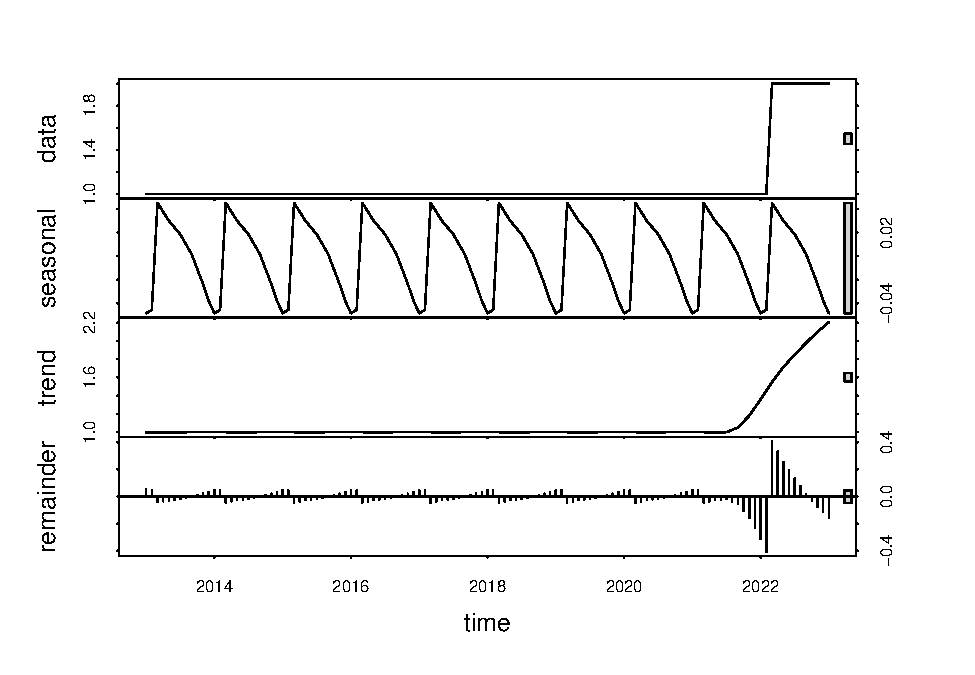
\includegraphics{Final-Project_files/figure-latex/unnamed-chunk-5-1.pdf}

\begin{Shaded}
\begin{Highlighting}[]
\FunctionTok{plot}\NormalTok{(decomp\_elec)}
\end{Highlighting}
\end{Shaded}

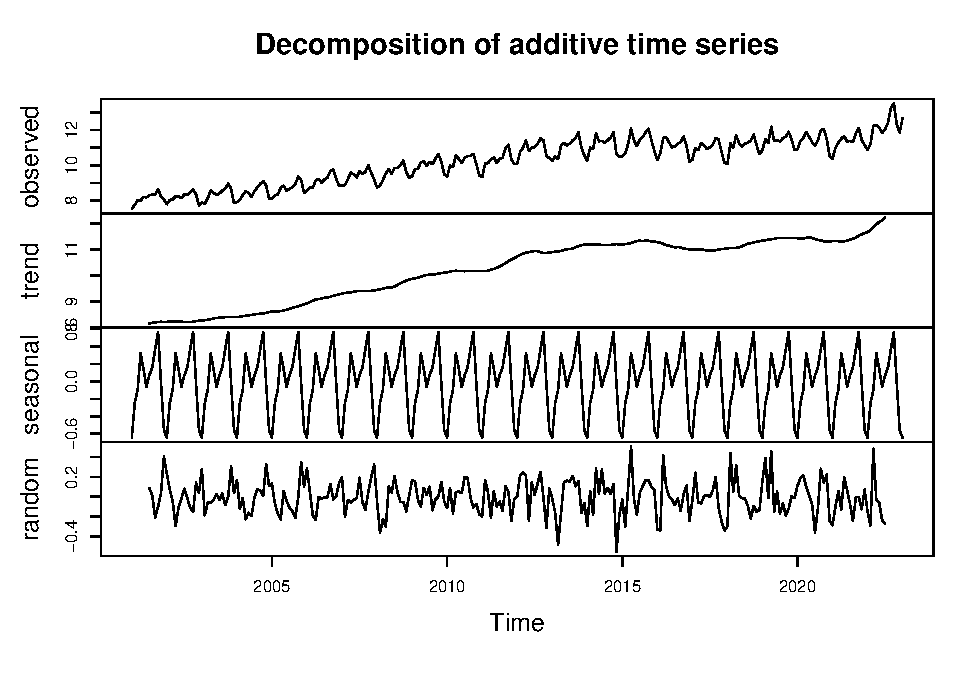
\includegraphics{Final-Project_files/figure-latex/unnamed-chunk-5-2.pdf}

\begin{Shaded}
\begin{Highlighting}[]
\CommentTok{\#remove seasonality}
\NormalTok{ts\_elec\_ns}\OtherTok{\textless{}{-}}\NormalTok{(ts\_electricity[,}\DecValTok{2}\NormalTok{] }\SpecialCharTok{{-}}\NormalTok{ decomp\_elec}\SpecialCharTok{$}\NormalTok{seasonal)}
\NormalTok{ts\_gas\_ns}\OtherTok{\textless{}{-}}\NormalTok{(ts\_gas\_equiv[,}\DecValTok{1}\NormalTok{] }\SpecialCharTok{{-}}\NormalTok{ decomp\_gas}\SpecialCharTok{$}\NormalTok{seasonal)}
\end{Highlighting}
\end{Shaded}

\hypertarget{plot-acf-and-pacf-to-see-the-general-pattern-of-two-series}{%
\subsection{plot ACF and PACF to see the general pattern of two
series}\label{plot-acf-and-pacf-to-see-the-general-pattern-of-two-series}}

\begin{Shaded}
\begin{Highlighting}[]
\CommentTok{\# ACF and PACF of electricity data}
\FunctionTok{par}\NormalTok{(}\AttributeTok{mfrow=}\FunctionTok{c}\NormalTok{(}\DecValTok{1}\NormalTok{,}\DecValTok{2}\NormalTok{))}
\FunctionTok{Acf}\NormalTok{(ts\_electricity[,}\DecValTok{2}\NormalTok{], }\AttributeTok{lag.max=}\DecValTok{40}\NormalTok{, }\AttributeTok{main=}\StringTok{"ACF Electricity"}\NormalTok{)}
\FunctionTok{Acf}\NormalTok{(ts\_elec\_ns, }\AttributeTok{lag.max=}\DecValTok{40}\NormalTok{, }\AttributeTok{main=}\StringTok{"ACF Non{-}Seasonal Electricity"}\NormalTok{)}
\end{Highlighting}
\end{Shaded}

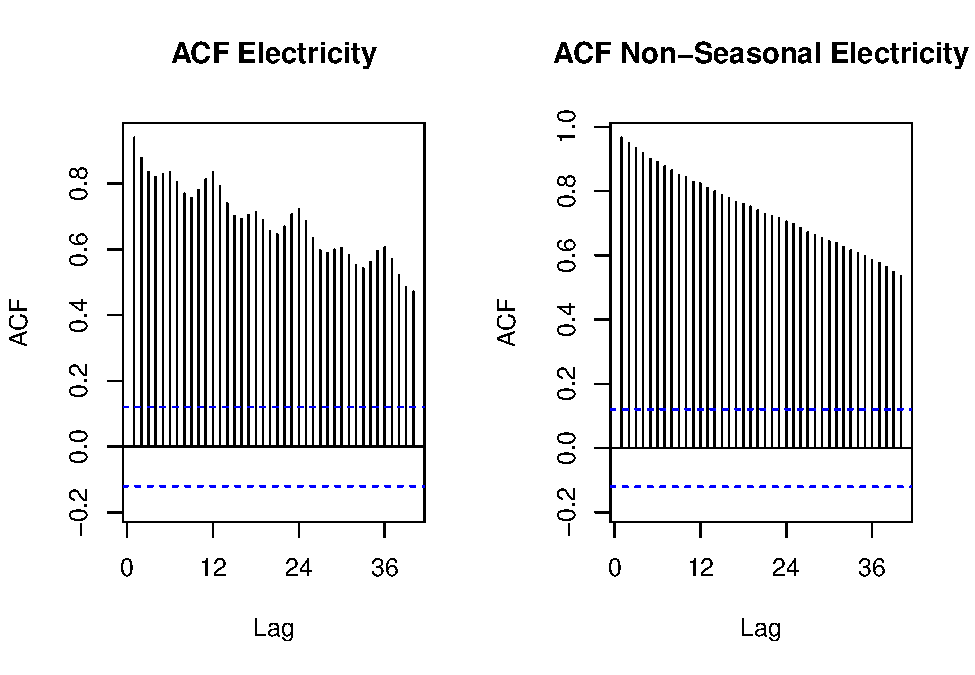
\includegraphics{Final-Project_files/figure-latex/unnamed-chunk-6-1.pdf}

\begin{Shaded}
\begin{Highlighting}[]
\FunctionTok{par}\NormalTok{(}\AttributeTok{mfrow=}\FunctionTok{c}\NormalTok{(}\DecValTok{1}\NormalTok{,}\DecValTok{2}\NormalTok{))}
\FunctionTok{Pacf}\NormalTok{(ts\_electricity[,}\DecValTok{2}\NormalTok{], }\AttributeTok{lag.max=}\DecValTok{40}\NormalTok{, }\AttributeTok{main=}\StringTok{"PACF Electricity"}\NormalTok{)}
\FunctionTok{Pacf}\NormalTok{(ts\_elec\_ns, }\AttributeTok{lag.max=}\DecValTok{40}\NormalTok{, }\AttributeTok{main=}\StringTok{"PACF Non{-}Seasonal Electricity"}\NormalTok{)}
\end{Highlighting}
\end{Shaded}

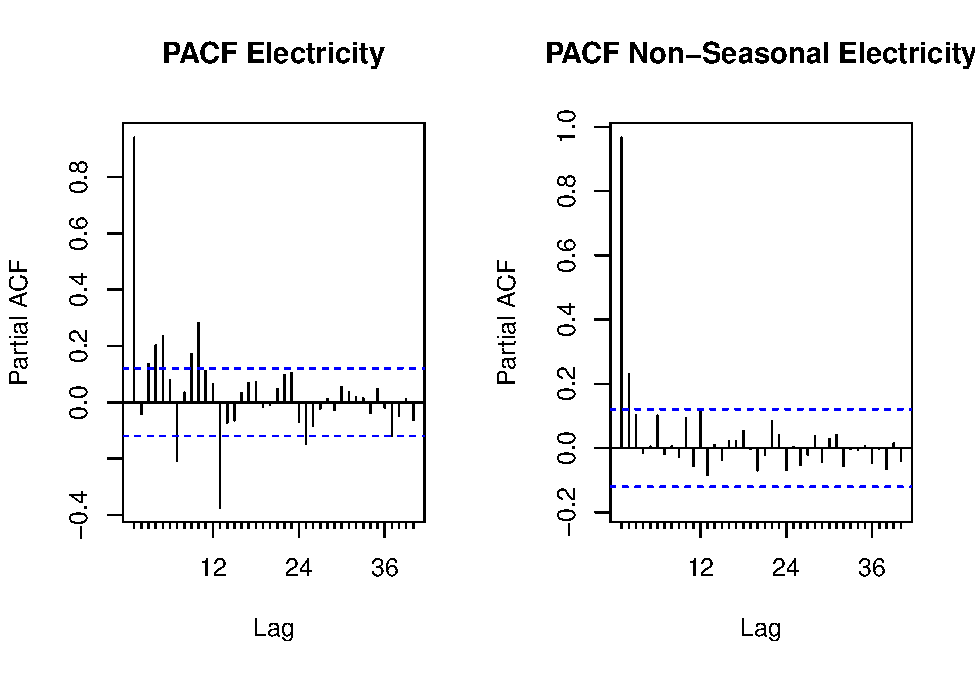
\includegraphics{Final-Project_files/figure-latex/unnamed-chunk-6-2.pdf}

\begin{Shaded}
\begin{Highlighting}[]
\CommentTok{\# ACF and PACF of natural gas data}
\FunctionTok{par}\NormalTok{(}\AttributeTok{mfrow=}\FunctionTok{c}\NormalTok{(}\DecValTok{1}\NormalTok{,}\DecValTok{2}\NormalTok{))}
\FunctionTok{Acf}\NormalTok{(ts\_gas\_equiv[,}\DecValTok{1}\NormalTok{], }\AttributeTok{lag.max=}\DecValTok{40}\NormalTok{, }\AttributeTok{main=}\StringTok{"ACF Natural Gas"}\NormalTok{)}
\FunctionTok{Acf}\NormalTok{(ts\_gas\_ns, }\AttributeTok{lag.max=}\DecValTok{40}\NormalTok{, }\AttributeTok{main=}\StringTok{"ACF Non{-}Seasonal Gas"}\NormalTok{)}
\end{Highlighting}
\end{Shaded}

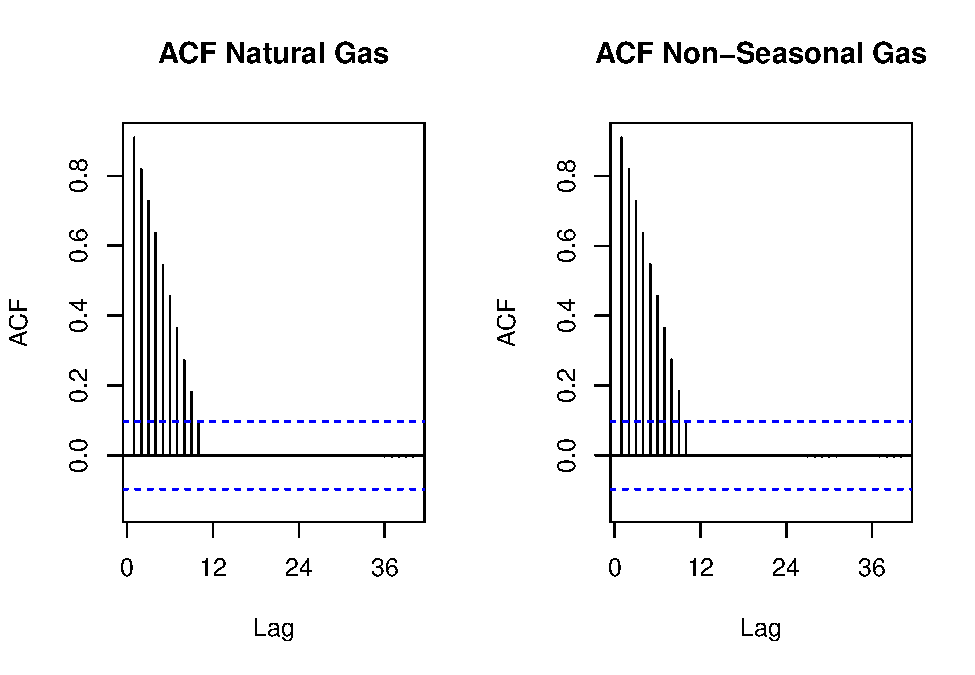
\includegraphics{Final-Project_files/figure-latex/unnamed-chunk-6-3.pdf}

\begin{Shaded}
\begin{Highlighting}[]
\FunctionTok{par}\NormalTok{(}\AttributeTok{mfrow=}\FunctionTok{c}\NormalTok{(}\DecValTok{1}\NormalTok{,}\DecValTok{2}\NormalTok{))}
\FunctionTok{Pacf}\NormalTok{(ts\_gas\_equiv[,}\DecValTok{1}\NormalTok{], }\AttributeTok{lag.max=}\DecValTok{40}\NormalTok{, }\AttributeTok{main=}\StringTok{"PACF Natural Gas"}\NormalTok{)}
\FunctionTok{Pacf}\NormalTok{(ts\_gas\_ns, }\AttributeTok{lag.max=}\DecValTok{40}\NormalTok{, }\AttributeTok{main=}\StringTok{"PACF Non{-}Seasonal Gas"}\NormalTok{)}
\end{Highlighting}
\end{Shaded}

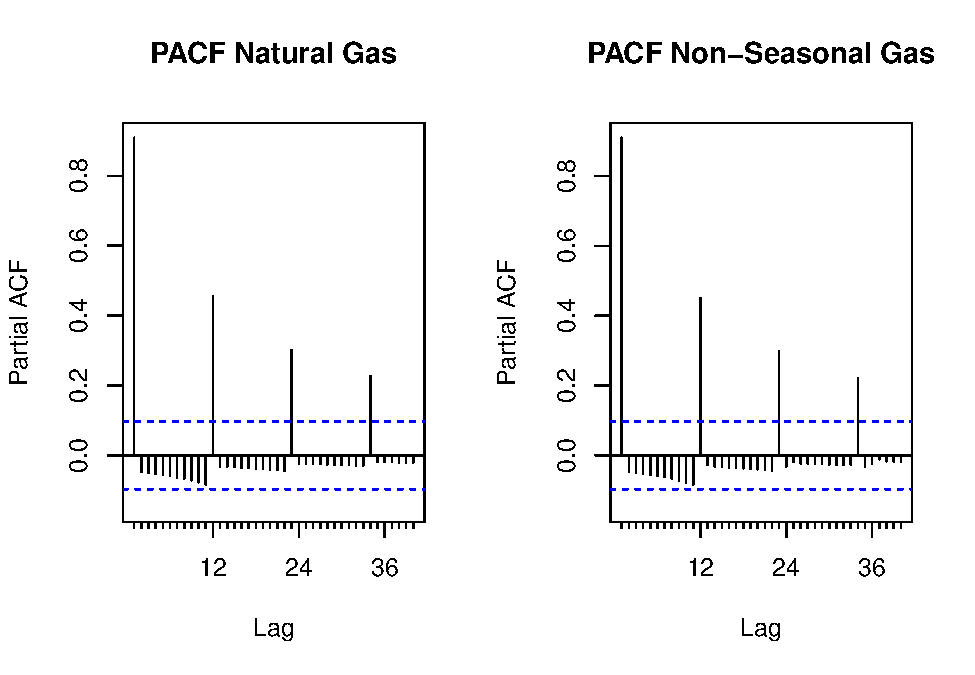
\includegraphics{Final-Project_files/figure-latex/unnamed-chunk-6-4.pdf}

\hypertarget{use-seasonal-arima-to-model-eletricity-and-natural-gas}{%
\subsection{Use seasonal Arima to model eletricity and natural
gas}\label{use-seasonal-arima-to-model-eletricity-and-natural-gas}}

\begin{Shaded}
\begin{Highlighting}[]
\CommentTok{\#forecast Electricity SARIMA}

\NormalTok{arima.e.model}\OtherTok{\textless{}{-}}\FunctionTok{auto.arima}\NormalTok{(}\FunctionTok{window}\NormalTok{(ts\_electricity[, }\DecValTok{2}\NormalTok{], }\AttributeTok{end=}\FunctionTok{c}\NormalTok{(}\DecValTok{2022}\NormalTok{,}\DecValTok{1}\NormalTok{)))}
\NormalTok{arima.e.forecast}\OtherTok{\textless{}{-}}\FunctionTok{forecast}\NormalTok{(arima.e.model, }\AttributeTok{h=}\DecValTok{12}\NormalTok{)}

\FunctionTok{autoplot}\NormalTok{(ts\_electricity[, }\DecValTok{2}\NormalTok{]) }\SpecialCharTok{+}
  \FunctionTok{autolayer}\NormalTok{(arima.e.forecast}\SpecialCharTok{$}\NormalTok{mean, }\AttributeTok{series =} \StringTok{"SARIMA"}\NormalTok{) }\SpecialCharTok{+}
  \FunctionTok{ylab}\NormalTok{(}\StringTok{"Price (cents/kWh)"}\NormalTok{) }\SpecialCharTok{+}
  \FunctionTok{ggtitle}\NormalTok{(}\StringTok{"Electricity {-} SARIMA"}\NormalTok{)}
\end{Highlighting}
\end{Shaded}

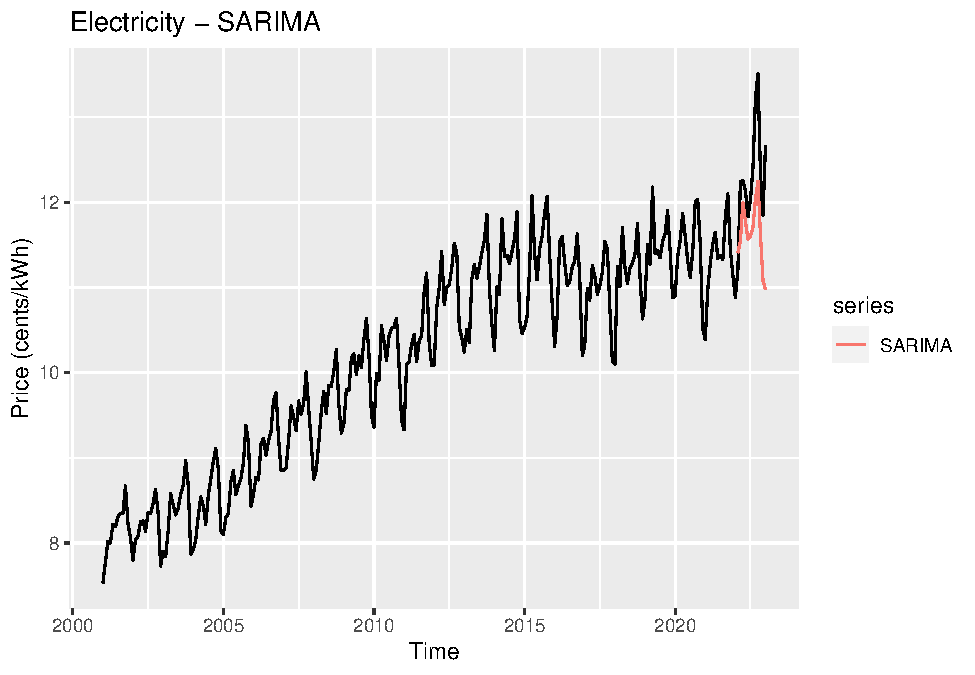
\includegraphics{Final-Project_files/figure-latex/unnamed-chunk-7-1.pdf}

\begin{Shaded}
\begin{Highlighting}[]
  \CommentTok{\# performance is not that good}

\CommentTok{\#Gas SARIMA forecast}
\NormalTok{arima.gas.model}\OtherTok{\textless{}{-}}\FunctionTok{auto.arima}\NormalTok{(}\FunctionTok{window}\NormalTok{(ts\_gas\_equiv[, }\DecValTok{1}\NormalTok{], }\AttributeTok{end=}\FunctionTok{c}\NormalTok{(}\DecValTok{2022}\NormalTok{,}\DecValTok{1}\NormalTok{)))}
\NormalTok{arima.gas.forecast}\OtherTok{\textless{}{-}}\FunctionTok{forecast}\NormalTok{(arima.gas.model, }\AttributeTok{h=}\DecValTok{12}\NormalTok{)}

\FunctionTok{autoplot}\NormalTok{(ts\_gas\_equiv[, }\DecValTok{1}\NormalTok{])}\SpecialCharTok{+}
  \FunctionTok{autolayer}\NormalTok{(arima.gas.forecast}\SpecialCharTok{$}\NormalTok{mean, }\AttributeTok{series =} \StringTok{"SARIMA"}\NormalTok{) }\SpecialCharTok{+}
  \FunctionTok{ylab}\NormalTok{(}\StringTok{"Price (cents/kWh)"}\NormalTok{) }\SpecialCharTok{+}
  \FunctionTok{ggtitle}\NormalTok{(}\StringTok{"Natural Gas {-} SARIMA"}\NormalTok{)}
\end{Highlighting}
\end{Shaded}

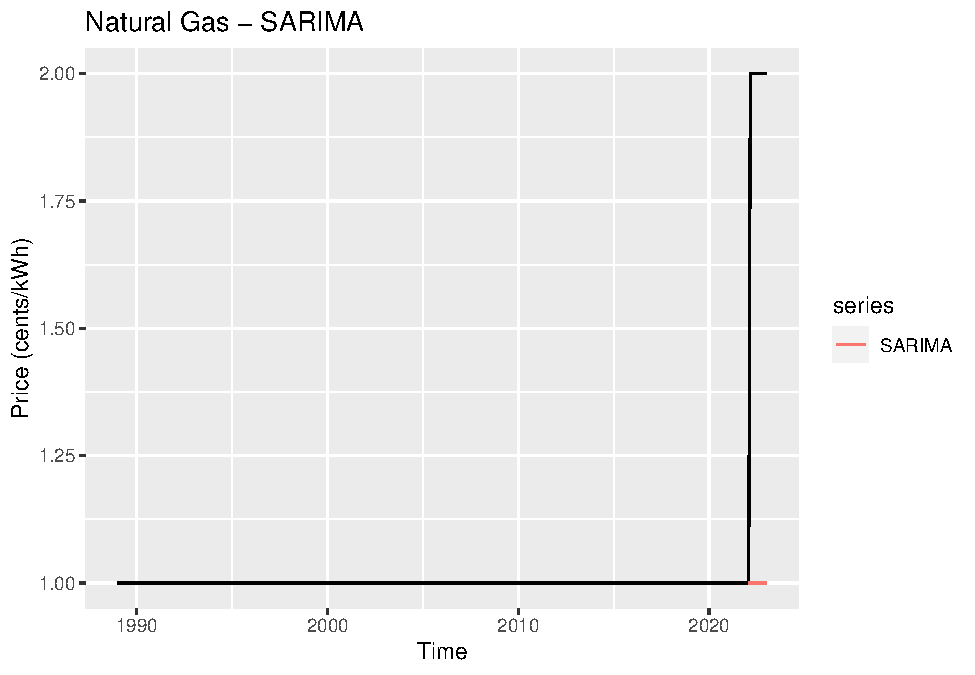
\includegraphics{Final-Project_files/figure-latex/unnamed-chunk-7-2.pdf}

\begin{Shaded}
\begin{Highlighting}[]
  \CommentTok{\# performance is not that good}
\end{Highlighting}
\end{Shaded}

\hypertarget{examine-seasonal-arima-models-performance-on-electricity-and-ng-data}{%
\subsubsection{Examine seasonal Arima model's performance on electricity
and NG
data}\label{examine-seasonal-arima-models-performance-on-electricity-and-ng-data}}

\begin{Shaded}
\begin{Highlighting}[]
\CommentTok{\# model performance for electricity data}
\NormalTok{sarima\_e\_perf }\OtherTok{\textless{}{-}}\NormalTok{ ts\_electricity[, }\DecValTok{2}\NormalTok{] }\SpecialCharTok{\%\textgreater{}\%} 
  \FunctionTok{window}\NormalTok{(}\AttributeTok{start =} \FunctionTok{c}\NormalTok{(}\DecValTok{2022}\NormalTok{, }\DecValTok{2}\NormalTok{)) }\SpecialCharTok{\%\textgreater{}\%} 
  \FunctionTok{accuracy}\NormalTok{(arima.e.forecast}\SpecialCharTok{$}\NormalTok{mean)}


\CommentTok{\# model performance for gas data}
\NormalTok{sarima\_gas\_perf }\OtherTok{\textless{}{-}}\NormalTok{ ts\_gas\_equiv[, }\DecValTok{1}\NormalTok{] }\SpecialCharTok{\%\textgreater{}\%} 
  \FunctionTok{window}\NormalTok{(}\AttributeTok{start =} \FunctionTok{c}\NormalTok{(}\DecValTok{2022}\NormalTok{, }\DecValTok{2}\NormalTok{)) }\SpecialCharTok{\%\textgreater{}\%} 
  \FunctionTok{accuracy}\NormalTok{(arima.gas.forecast}\SpecialCharTok{$}\NormalTok{mean)}
\end{Highlighting}
\end{Shaded}

\hypertarget{use-arima-with-fourier-terms-to-model}{%
\subsection{Use Arima with Fourier terms to
model}\label{use-arima-with-fourier-terms-to-model}}

\begin{Shaded}
\begin{Highlighting}[]
\CommentTok{\# arima with fourier terms for eletricity}
\NormalTok{arima.e.four.forecast }\OtherTok{\textless{}{-}}\NormalTok{ ts\_electricity[, }\DecValTok{2}\NormalTok{] }\SpecialCharTok{\%\textgreater{}\%} 
  \FunctionTok{window}\NormalTok{(}\AttributeTok{end =} \FunctionTok{c}\NormalTok{(}\DecValTok{2022}\NormalTok{, }\DecValTok{1}\NormalTok{)) }\SpecialCharTok{\%\textgreater{}\%} 
  \FunctionTok{auto.arima}\NormalTok{(}\AttributeTok{seasonal =} \ConstantTok{FALSE}\NormalTok{, }
             \AttributeTok{xreg =} \FunctionTok{fourier}\NormalTok{(}\FunctionTok{window}\NormalTok{(ts\_electricity[, }\DecValTok{2}\NormalTok{], }\AttributeTok{end =} \FunctionTok{c}\NormalTok{(}\DecValTok{2022}\NormalTok{, }\DecValTok{1}\NormalTok{)), }
                            \AttributeTok{K =} \DecValTok{6}\NormalTok{)) }\SpecialCharTok{\%\textgreater{}\%} 
  \FunctionTok{forecast}\NormalTok{(}\AttributeTok{xreg =} \FunctionTok{fourier}\NormalTok{(}\FunctionTok{window}\NormalTok{(ts\_electricity[, }\DecValTok{2}\NormalTok{], }
                                 \AttributeTok{start =} \FunctionTok{c}\NormalTok{(}\DecValTok{2022}\NormalTok{,}\DecValTok{2}\NormalTok{)}
\NormalTok{                                 ),}
                            \AttributeTok{K =} \DecValTok{6}\NormalTok{),}
           \AttributeTok{h =} \DecValTok{12}\NormalTok{)}

\FunctionTok{autoplot}\NormalTok{(arima.e.four.forecast}\SpecialCharTok{$}\NormalTok{mean, }\AttributeTok{series =} \StringTok{"ARIMA with Fourier Terms"}\NormalTok{) }\SpecialCharTok{+}
  \FunctionTok{autolayer}\NormalTok{(ts\_electricity[, }\DecValTok{2}\NormalTok{], }\AttributeTok{series =} \StringTok{"Historical Data"}\NormalTok{) }\SpecialCharTok{+}
  \FunctionTok{ggtitle}\NormalTok{(}\StringTok{"Electricity {-} ARIMA with Fourier Terms"}\NormalTok{) }\SpecialCharTok{+}
  \FunctionTok{ylab}\NormalTok{(}\StringTok{"Price (cents/kWh)"}\NormalTok{)}
\end{Highlighting}
\end{Shaded}

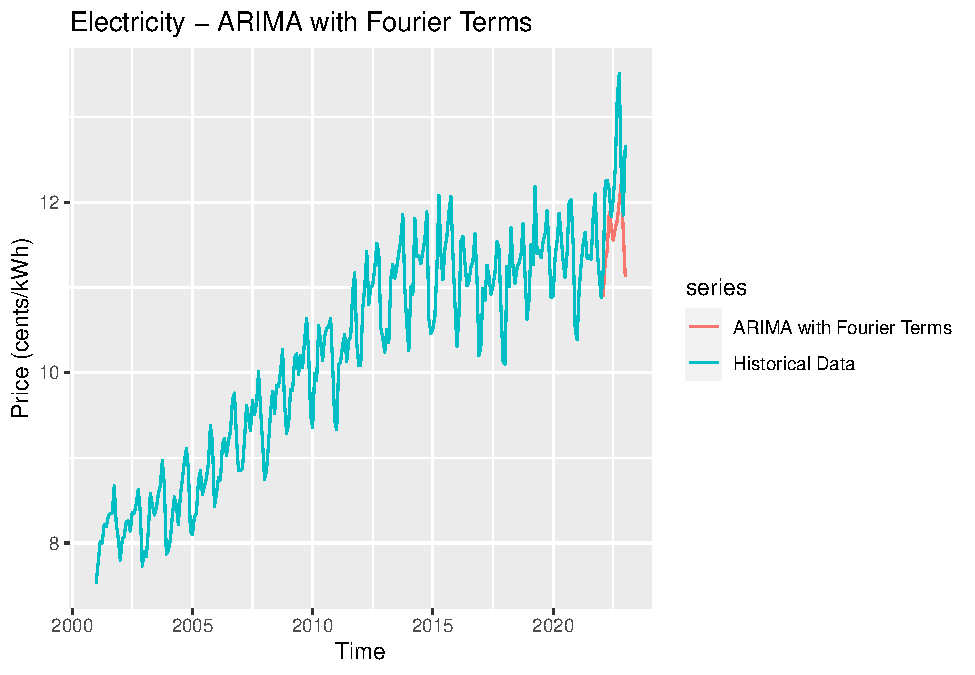
\includegraphics{Final-Project_files/figure-latex/unnamed-chunk-9-1.pdf}

\begin{Shaded}
\begin{Highlighting}[]
\CommentTok{\# arima with fourier terms for gas}
\NormalTok{arima.gas.four.forecast }\OtherTok{\textless{}{-}}\NormalTok{ ts\_gas\_equiv[, }\DecValTok{1}\NormalTok{] }\SpecialCharTok{\%\textgreater{}\%} 
  \FunctionTok{window}\NormalTok{(}\AttributeTok{end =} \FunctionTok{c}\NormalTok{(}\DecValTok{2022}\NormalTok{, }\DecValTok{1}\NormalTok{)) }\SpecialCharTok{\%\textgreater{}\%} 
  \FunctionTok{auto.arima}\NormalTok{(}\AttributeTok{seasonal =} \ConstantTok{FALSE}\NormalTok{,}
             \AttributeTok{xreg =} \FunctionTok{fourier}\NormalTok{(}\FunctionTok{window}\NormalTok{(ts\_gas\_equiv[, }\DecValTok{1}\NormalTok{], }\AttributeTok{end =} \FunctionTok{c}\NormalTok{(}\DecValTok{2022}\NormalTok{, }\DecValTok{1}\NormalTok{)), }
                            \AttributeTok{K =} \DecValTok{6}\NormalTok{)}
\NormalTok{             ) }\SpecialCharTok{\%\textgreater{}\%} 
  \FunctionTok{forecast}\NormalTok{(}\AttributeTok{xreg =} \FunctionTok{fourier}\NormalTok{(}\FunctionTok{window}\NormalTok{(ts\_gas\_equiv[, }\DecValTok{1}\NormalTok{], }
                                 \AttributeTok{start =} \FunctionTok{c}\NormalTok{(}\DecValTok{2022}\NormalTok{, }\DecValTok{2}\NormalTok{)}
\NormalTok{                                 ),}
                          \AttributeTok{K =} \DecValTok{6}\NormalTok{), }
           \AttributeTok{h =} \DecValTok{12}\NormalTok{)}

\FunctionTok{autoplot}\NormalTok{(arima.gas.four.forecast}\SpecialCharTok{$}\NormalTok{mean, }\AttributeTok{series =} \StringTok{"ARIMA with Fourier Terms"}\NormalTok{) }\SpecialCharTok{+}
  \FunctionTok{autolayer}\NormalTok{(ts\_gas\_equiv[, }\DecValTok{1}\NormalTok{], }\AttributeTok{series =} \StringTok{"Historical Data"}\NormalTok{) }\SpecialCharTok{+}
  \FunctionTok{ggtitle}\NormalTok{(}\StringTok{"Natural Gas {-} ARIMA with Fourier Terms"}\NormalTok{) }\SpecialCharTok{+}
  \FunctionTok{ylab}\NormalTok{(}\StringTok{"Price (cents/kWh)"}\NormalTok{)}
\end{Highlighting}
\end{Shaded}

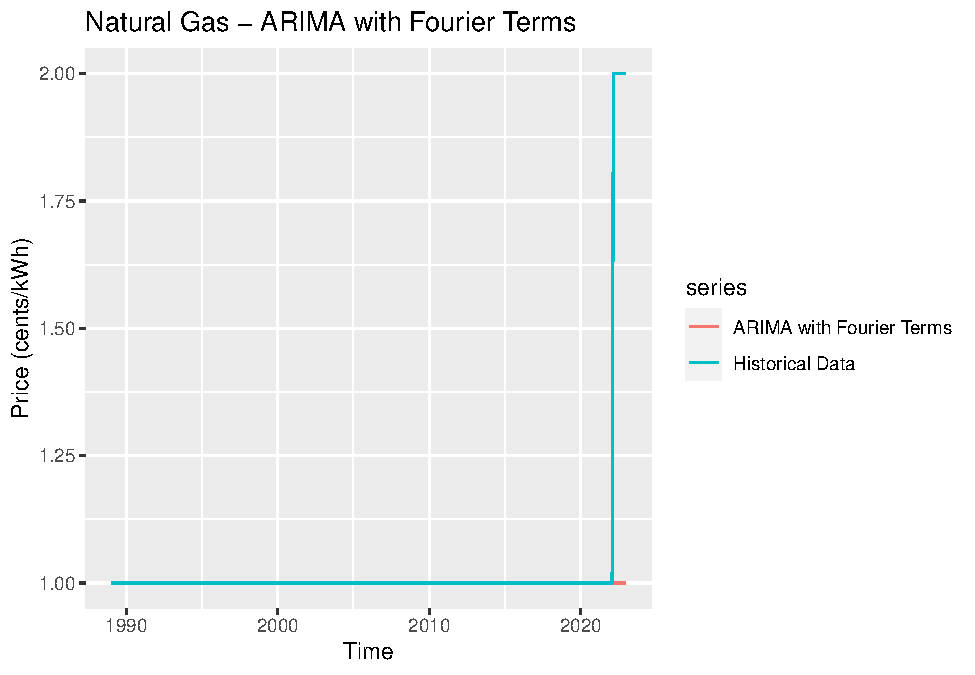
\includegraphics{Final-Project_files/figure-latex/unnamed-chunk-9-2.pdf}

\hypertarget{examine-arima-with-fouriers-performance-on-electricity-and-ng-data}{%
\subsubsection{Examine Arima with fourier's performance on electricity
and NG
data}\label{examine-arima-with-fouriers-performance-on-electricity-and-ng-data}}

\begin{Shaded}
\begin{Highlighting}[]
\CommentTok{\# model performance for electricity data}
\NormalTok{arima\_four\_e\_perf }\OtherTok{\textless{}{-}}\NormalTok{ ts\_electricity[, }\DecValTok{2}\NormalTok{] }\SpecialCharTok{\%\textgreater{}\%} 
  \FunctionTok{window}\NormalTok{(}\AttributeTok{start =} \FunctionTok{c}\NormalTok{(}\DecValTok{2022}\NormalTok{, }\DecValTok{2}\NormalTok{)) }\SpecialCharTok{\%\textgreater{}\%} 
  \FunctionTok{accuracy}\NormalTok{(arima.e.four.forecast}\SpecialCharTok{$}\NormalTok{mean)}

\CommentTok{\# model performance for gas data}
\NormalTok{arima\_four\_gas\_perf }\OtherTok{\textless{}{-}}\NormalTok{ ts\_gas\_equiv[, }\DecValTok{1}\NormalTok{] }\SpecialCharTok{\%\textgreater{}\%} 
  \FunctionTok{window}\NormalTok{(}\AttributeTok{start =} \FunctionTok{c}\NormalTok{(}\DecValTok{2022}\NormalTok{, }\DecValTok{2}\NormalTok{)) }\SpecialCharTok{\%\textgreater{}\%} 
  \FunctionTok{accuracy}\NormalTok{(arima.gas.four.forecast}\SpecialCharTok{$}\NormalTok{mean)}
\end{Highlighting}
\end{Shaded}

\hypertarget{use-stl-to-model}{%
\subsection{Use STL to model}\label{use-stl-to-model}}

\begin{Shaded}
\begin{Highlighting}[]
\CommentTok{\# STL for electricity}
\NormalTok{stl.e.forecast }\OtherTok{\textless{}{-}}\NormalTok{ ts\_electricity[, }\DecValTok{2}\NormalTok{] }\SpecialCharTok{\%\textgreater{}\%} 
  \FunctionTok{window}\NormalTok{(}\AttributeTok{end =} \FunctionTok{c}\NormalTok{(}\DecValTok{2022}\NormalTok{, }\DecValTok{1}\NormalTok{)) }\SpecialCharTok{\%\textgreater{}\%} 
  \FunctionTok{stlf}\NormalTok{(}\AttributeTok{h =} \DecValTok{12}\NormalTok{)}

\FunctionTok{autoplot}\NormalTok{(stl.e.forecast}\SpecialCharTok{$}\NormalTok{mean, }\AttributeTok{series =} \StringTok{"STL + ETS"}\NormalTok{) }\SpecialCharTok{+}
  \FunctionTok{autolayer}\NormalTok{(ts\_electricity[, }\DecValTok{2}\NormalTok{], }\AttributeTok{series =} \StringTok{"Historical Data"}\NormalTok{) }\SpecialCharTok{+}
  \FunctionTok{ggtitle}\NormalTok{(}\StringTok{"Electricity {-} STL + EST"}\NormalTok{) }\SpecialCharTok{+}
  \FunctionTok{ylab}\NormalTok{(}\StringTok{"Price (cents/kWh)"}\NormalTok{)}
\end{Highlighting}
\end{Shaded}

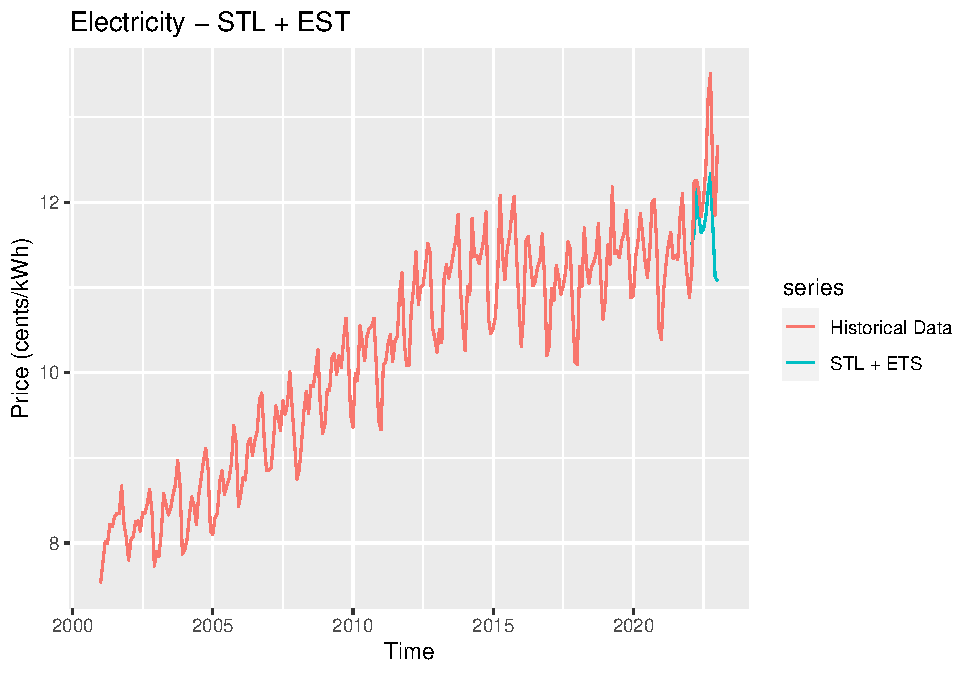
\includegraphics{Final-Project_files/figure-latex/unnamed-chunk-11-1.pdf}

\begin{Shaded}
\begin{Highlighting}[]
\CommentTok{\# STL for gas}
\NormalTok{stl.gas.forecast }\OtherTok{\textless{}{-}}\NormalTok{ ts\_gas\_equiv[, }\DecValTok{1}\NormalTok{] }\SpecialCharTok{\%\textgreater{}\%} 
  \FunctionTok{window}\NormalTok{(}\AttributeTok{end =} \FunctionTok{c}\NormalTok{(}\DecValTok{2022}\NormalTok{, }\DecValTok{1}\NormalTok{)) }\SpecialCharTok{\%\textgreater{}\%} 
  \FunctionTok{stlf}\NormalTok{(}\AttributeTok{h =} \DecValTok{12}\NormalTok{)}

\FunctionTok{autoplot}\NormalTok{(ts\_gas\_equiv[, }\DecValTok{1}\NormalTok{], }\AttributeTok{series =} \StringTok{"Historical Data"}\NormalTok{) }\SpecialCharTok{+}
  \FunctionTok{autolayer}\NormalTok{(stl.gas.forecast}\SpecialCharTok{$}\NormalTok{mean, }\AttributeTok{series =} \StringTok{"STL + ETS"}\NormalTok{) }\SpecialCharTok{+}
  \FunctionTok{ggtitle}\NormalTok{(}\StringTok{"Natural Gas {-} STL + EST"}\NormalTok{) }\SpecialCharTok{+}
  \FunctionTok{ylab}\NormalTok{(}\StringTok{"Price (cents/kWh)"}\NormalTok{)}
\end{Highlighting}
\end{Shaded}

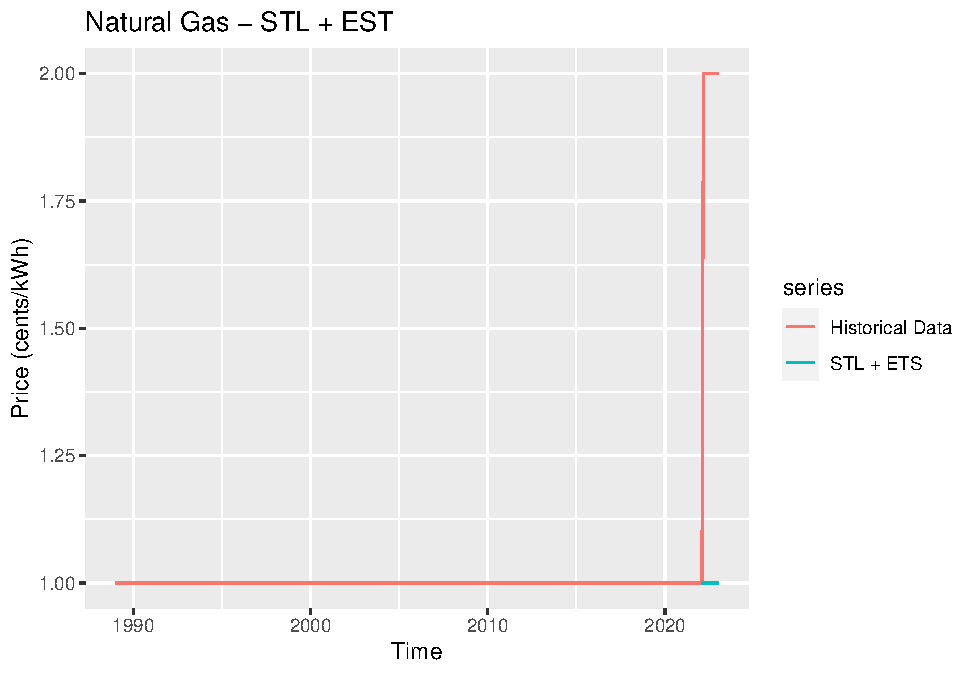
\includegraphics{Final-Project_files/figure-latex/unnamed-chunk-11-2.pdf}

\hypertarget{examine-stls-performance-on-electricity-and-ng-data}{%
\subsubsection{Examine STL's performance on electricity and NG
data}\label{examine-stls-performance-on-electricity-and-ng-data}}

\begin{Shaded}
\begin{Highlighting}[]
\CommentTok{\# model performance for electricity data}
\NormalTok{stl\_e\_perf }\OtherTok{\textless{}{-}}\NormalTok{ ts\_electricity[, }\DecValTok{2}\NormalTok{] }\SpecialCharTok{\%\textgreater{}\%} 
  \FunctionTok{window}\NormalTok{(}\AttributeTok{start =} \FunctionTok{c}\NormalTok{(}\DecValTok{2022}\NormalTok{, }\DecValTok{2}\NormalTok{)) }\SpecialCharTok{\%\textgreater{}\%} 
  \FunctionTok{accuracy}\NormalTok{(stl.e.forecast}\SpecialCharTok{$}\NormalTok{mean)}

\CommentTok{\# model performance for gas data}
\NormalTok{stl\_gas\_perf }\OtherTok{\textless{}{-}}\NormalTok{ ts\_gas\_equiv[, }\DecValTok{1}\NormalTok{] }\SpecialCharTok{\%\textgreater{}\%} 
  \FunctionTok{window}\NormalTok{(}\AttributeTok{start =} \FunctionTok{c}\NormalTok{(}\DecValTok{2022}\NormalTok{, }\DecValTok{2}\NormalTok{)) }\SpecialCharTok{\%\textgreater{}\%} 
  \FunctionTok{accuracy}\NormalTok{(stl.gas.forecast}\SpecialCharTok{$}\NormalTok{mean)}
\end{Highlighting}
\end{Shaded}

\hypertarget{use-ets-to-model-not-finished-i-dont-know-how-to-do-this}{%
\subsection{Use ETS to model -- not finished -- I don't know how to do
this}\label{use-ets-to-model-not-finished-i-dont-know-how-to-do-this}}

\begin{Shaded}
\begin{Highlighting}[]
\CommentTok{\# I think STL doesn\textquotesingle{}t need fourier terms. So, I will get covariates dataframes without fourier terms}
\CommentTok{\# because UKRWAR and temperature are the same across two data frames, we only need one}
\NormalTok{cov\_train\_nofour }\OtherTok{\textless{}{-}}\NormalTok{ covariates\_train\_e[, }\DecValTok{1}\SpecialCharTok{:}\DecValTok{2}\NormalTok{]}
\FunctionTok{colnames}\NormalTok{(cov\_train\_nofour) }\OtherTok{\textless{}{-}} \FunctionTok{c}\NormalTok{(}\StringTok{"UKRWAR"}\NormalTok{, }\StringTok{"temperature"}\NormalTok{)}

\NormalTok{cov\_test\_nofour }\OtherTok{\textless{}{-}}\NormalTok{ covariates\_full\_e[, }\DecValTok{1}\SpecialCharTok{:}\DecValTok{2}\NormalTok{] }\SpecialCharTok{\%\textgreater{}\%} 
  \FunctionTok{window}\NormalTok{(}\AttributeTok{start =} \FunctionTok{c}\NormalTok{(}\DecValTok{2022}\NormalTok{, }\DecValTok{2}\NormalTok{))}
\FunctionTok{colnames}\NormalTok{(cov\_test\_nofour) }\OtherTok{\textless{}{-}} \FunctionTok{c}\NormalTok{(}\StringTok{"UKRWAR"}\NormalTok{, }\StringTok{"temperature"}\NormalTok{)}
\end{Highlighting}
\end{Shaded}

\hypertarget{use-neural-network-and-fourier-to-model}{%
\subsection{Use Neural Network and fourier to
model}\label{use-neural-network-and-fourier-to-model}}

\begin{Shaded}
\begin{Highlighting}[]
\CommentTok{\# neural network forecast for electricity data}
\NormalTok{nn.e.forecast }\OtherTok{\textless{}{-}}\NormalTok{ ts\_electricity[, }\DecValTok{2}\NormalTok{] }\SpecialCharTok{\%\textgreater{}\%} 
  \FunctionTok{window}\NormalTok{(}\AttributeTok{end =} \FunctionTok{c}\NormalTok{(}\DecValTok{2022}\NormalTok{ ,}\DecValTok{1}\NormalTok{)) }\SpecialCharTok{\%\textgreater{}\%} 
  \FunctionTok{nnetar}\NormalTok{(}\AttributeTok{p =} \DecValTok{2}\NormalTok{, }\AttributeTok{P =} \DecValTok{1}\NormalTok{, }\CommentTok{\# 2 and 1 are randomly decided. To find the optimal one, }
         \CommentTok{\# we need to run a couple of combinations to find the best one}
         \AttributeTok{xreg =} \FunctionTok{fourier}\NormalTok{(}\FunctionTok{window}\NormalTok{(ts\_electricity[, }\DecValTok{2}\NormalTok{], }
                               \AttributeTok{end =} \FunctionTok{c}\NormalTok{(}\DecValTok{2022}\NormalTok{, }\DecValTok{1}\NormalTok{)}
\NormalTok{                               ),}
                        \AttributeTok{K =} \DecValTok{6}\NormalTok{)}
\NormalTok{         ) }\SpecialCharTok{\%\textgreater{}\%} 
  \FunctionTok{forecast}\NormalTok{(}\AttributeTok{xreg =} \FunctionTok{fourier}\NormalTok{(}\FunctionTok{window}\NormalTok{(ts\_electricity[, }\DecValTok{2}\NormalTok{], }
                                 \AttributeTok{start =} \FunctionTok{c}\NormalTok{(}\DecValTok{2022}\NormalTok{, }\DecValTok{2}\NormalTok{)}
\NormalTok{                                 ),}
                          \AttributeTok{K =} \DecValTok{6}\NormalTok{),}
           \AttributeTok{h =} \DecValTok{12}\NormalTok{)}

\CommentTok{\# neural network forecast for gas data}
\NormalTok{nn.gas.forecast }\OtherTok{\textless{}{-}}\NormalTok{ ts\_gas\_equiv[, }\DecValTok{1}\NormalTok{] }\SpecialCharTok{\%\textgreater{}\%} 
  \FunctionTok{window}\NormalTok{(}\AttributeTok{end =} \FunctionTok{c}\NormalTok{(}\DecValTok{2022}\NormalTok{ ,}\DecValTok{1}\NormalTok{)) }\SpecialCharTok{\%\textgreater{}\%} 
  \FunctionTok{nnetar}\NormalTok{(}\AttributeTok{p =} \DecValTok{2}\NormalTok{, }\AttributeTok{P =} \DecValTok{1}\NormalTok{,}
         \AttributeTok{xreg =} \FunctionTok{fourier}\NormalTok{(}\FunctionTok{window}\NormalTok{(ts\_gas\_equiv[, }\DecValTok{1}\NormalTok{], }
                               \AttributeTok{end =} \FunctionTok{c}\NormalTok{(}\DecValTok{2022}\NormalTok{, }\DecValTok{1}\NormalTok{)}
\NormalTok{                               ),}
                        \AttributeTok{K =} \DecValTok{6}\NormalTok{)}
\NormalTok{         ) }\SpecialCharTok{\%\textgreater{}\%} 
  \FunctionTok{forecast}\NormalTok{(}\AttributeTok{xreg =} \FunctionTok{fourier}\NormalTok{(}\FunctionTok{window}\NormalTok{(ts\_gas\_equiv[, }\DecValTok{1}\NormalTok{], }
                                 \AttributeTok{start =} \FunctionTok{c}\NormalTok{(}\DecValTok{2022}\NormalTok{, }\DecValTok{2}\NormalTok{)}
\NormalTok{                                 ),}
                          \AttributeTok{K =} \DecValTok{6}\NormalTok{),}
           \AttributeTok{h =} \DecValTok{12}\NormalTok{)}


\FunctionTok{autoplot}\NormalTok{(nn.e.forecast}\SpecialCharTok{$}\NormalTok{mean, }\AttributeTok{series =} \StringTok{"Neural Network"}\NormalTok{) }\SpecialCharTok{+}
  \FunctionTok{autolayer}\NormalTok{(ts\_electricity[, }\DecValTok{2}\NormalTok{], }\AttributeTok{series =} \StringTok{"Historical Data"}\NormalTok{) }\SpecialCharTok{+}
  \FunctionTok{ggtitle}\NormalTok{(}\StringTok{"Electricity {-} Neural Network"}\NormalTok{) }\SpecialCharTok{+}
  \FunctionTok{ylab}\NormalTok{(}\StringTok{"Price (cents/kWh)"}\NormalTok{)}
\end{Highlighting}
\end{Shaded}

\includegraphics{Final-Project_files/figure-latex/unnamed-chunk-14-1.pdf}

\begin{Shaded}
\begin{Highlighting}[]
\FunctionTok{autoplot}\NormalTok{(nn.gas.forecast}\SpecialCharTok{$}\NormalTok{mean, }\AttributeTok{series =} \StringTok{"Neural Network"}\NormalTok{) }\SpecialCharTok{+}
  \FunctionTok{autolayer}\NormalTok{(ts\_gas\_equiv[, }\DecValTok{1}\NormalTok{], }\AttributeTok{series =} \StringTok{"Historical Data"}\NormalTok{) }\SpecialCharTok{+}
  \FunctionTok{ggtitle}\NormalTok{(}\StringTok{"Natural Gas {-} Neural Network"}\NormalTok{) }\SpecialCharTok{+}
  \FunctionTok{ylab}\NormalTok{(}\StringTok{"Price (cents/kWh)"}\NormalTok{)}
\end{Highlighting}
\end{Shaded}

\includegraphics{Final-Project_files/figure-latex/unnamed-chunk-14-2.pdf}

\hypertarget{neutral-network-model-performance}{%
\subsubsection{neutral network model
performance}\label{neutral-network-model-performance}}

\begin{Shaded}
\begin{Highlighting}[]
\CommentTok{\# neural network model performance for electricity data}
\NormalTok{nn\_e\_perf }\OtherTok{\textless{}{-}}\NormalTok{ ts\_electricity[, }\DecValTok{2}\NormalTok{] }\SpecialCharTok{\%\textgreater{}\%} 
  \FunctionTok{window}\NormalTok{(}\AttributeTok{start =} \FunctionTok{c}\NormalTok{(}\DecValTok{2022}\NormalTok{, }\DecValTok{2}\NormalTok{)) }\SpecialCharTok{\%\textgreater{}\%} 
  \FunctionTok{accuracy}\NormalTok{(nn.e.forecast}\SpecialCharTok{$}\NormalTok{mean)}

\CommentTok{\# neural network model performance for gas data}
\NormalTok{nn\_gas\_perf }\OtherTok{\textless{}{-}}\NormalTok{ ts\_gas\_equiv[, }\DecValTok{1}\NormalTok{] }\SpecialCharTok{\%\textgreater{}\%} 
  \FunctionTok{window}\NormalTok{(}\AttributeTok{start =} \FunctionTok{c}\NormalTok{(}\DecValTok{2022}\NormalTok{, }\DecValTok{2}\NormalTok{)) }\SpecialCharTok{\%\textgreater{}\%} 
  \FunctionTok{accuracy}\NormalTok{(nn.gas.forecast}\SpecialCharTok{$}\NormalTok{mean)}
\end{Highlighting}
\end{Shaded}

\hypertarget{find-the-optimal-p-and-p-values-for-neural-network-without-fourier}{%
\subsection{find the optimal p and P values for neural network without
fourier}\label{find-the-optimal-p-and-p-values-for-neural-network-without-fourier}}

\begin{Shaded}
\begin{Highlighting}[]
\DocumentationTok{\#\# p = 1, P = 0}
\NormalTok{nn.e.forecast}\FloatTok{.10} \OtherTok{\textless{}{-}}\NormalTok{ ts\_electricity[, }\DecValTok{2}\NormalTok{] }\SpecialCharTok{\%\textgreater{}\%} 
  \FunctionTok{window}\NormalTok{(}\AttributeTok{end =} \FunctionTok{c}\NormalTok{(}\DecValTok{2022}\NormalTok{ ,}\DecValTok{1}\NormalTok{)) }\SpecialCharTok{\%\textgreater{}\%} 
  \FunctionTok{nnetar}\NormalTok{(}\AttributeTok{p =} \DecValTok{1}\NormalTok{, }\AttributeTok{P =} \DecValTok{0}\NormalTok{, }\CommentTok{\# 2 and 1 are randomly decided. To find the optimal one, }
         \CommentTok{\# we need to run a couple of combinations to find the best one}
\NormalTok{         ) }\SpecialCharTok{\%\textgreater{}\%} 
  \FunctionTok{forecast}\NormalTok{(}\AttributeTok{h =} \DecValTok{12}\NormalTok{)}

\NormalTok{nn.e.}\FloatTok{10.}\NormalTok{score }\OtherTok{\textless{}{-}}\NormalTok{ ts\_electricity[, }\DecValTok{2}\NormalTok{] }\SpecialCharTok{\%\textgreater{}\%} 
  \FunctionTok{window}\NormalTok{(}\AttributeTok{start =} \FunctionTok{c}\NormalTok{(}\DecValTok{2022}\NormalTok{, }\DecValTok{2}\NormalTok{)) }\SpecialCharTok{\%\textgreater{}\%} 
  \FunctionTok{accuracy}\NormalTok{(nn.e.forecast}\FloatTok{.10}\SpecialCharTok{$}\NormalTok{mean)}

\DocumentationTok{\#\# p = 1, P = 1}
\NormalTok{nn.e.forecast}\FloatTok{.11} \OtherTok{\textless{}{-}}\NormalTok{ ts\_electricity[, }\DecValTok{2}\NormalTok{] }\SpecialCharTok{\%\textgreater{}\%} 
  \FunctionTok{window}\NormalTok{(}\AttributeTok{end =} \FunctionTok{c}\NormalTok{(}\DecValTok{2022}\NormalTok{ ,}\DecValTok{1}\NormalTok{)) }\SpecialCharTok{\%\textgreater{}\%} 
  \FunctionTok{nnetar}\NormalTok{(}\AttributeTok{p =} \DecValTok{1}\NormalTok{, }\AttributeTok{P =} \DecValTok{1}\NormalTok{, }\CommentTok{\# 2 and 1 are randomly decided. To find the optimal one, }
         \CommentTok{\# we need to run a couple of combinations to find the best one}
\NormalTok{         ) }\SpecialCharTok{\%\textgreater{}\%} 
  \FunctionTok{forecast}\NormalTok{(}\AttributeTok{h =} \DecValTok{12}\NormalTok{)}

\NormalTok{nn.e.}\FloatTok{11.}\NormalTok{score }\OtherTok{\textless{}{-}}\NormalTok{ ts\_electricity[, }\DecValTok{2}\NormalTok{] }\SpecialCharTok{\%\textgreater{}\%} 
  \FunctionTok{window}\NormalTok{(}\AttributeTok{start =} \FunctionTok{c}\NormalTok{(}\DecValTok{2022}\NormalTok{, }\DecValTok{2}\NormalTok{)) }\SpecialCharTok{\%\textgreater{}\%} 
  \FunctionTok{accuracy}\NormalTok{(nn.e.forecast}\FloatTok{.11}\SpecialCharTok{$}\NormalTok{mean)}

\DocumentationTok{\#\# p = 2, P = 0}
\NormalTok{nn.e.forecast}\FloatTok{.20} \OtherTok{\textless{}{-}}\NormalTok{ ts\_electricity[, }\DecValTok{2}\NormalTok{] }\SpecialCharTok{\%\textgreater{}\%} 
  \FunctionTok{window}\NormalTok{(}\AttributeTok{end =} \FunctionTok{c}\NormalTok{(}\DecValTok{2022}\NormalTok{ ,}\DecValTok{1}\NormalTok{)) }\SpecialCharTok{\%\textgreater{}\%} 
  \FunctionTok{nnetar}\NormalTok{(}\AttributeTok{p =} \DecValTok{2}\NormalTok{, }\AttributeTok{P =} \DecValTok{0}\NormalTok{, }\CommentTok{\# 2 and 1 are randomly decided. To find the optimal one, }
         \CommentTok{\# we need to run a couple of combinations to find the best one}
\NormalTok{         ) }\SpecialCharTok{\%\textgreater{}\%} 
  \FunctionTok{forecast}\NormalTok{(}\AttributeTok{h =} \DecValTok{12}\NormalTok{)}

\NormalTok{nn.e.}\FloatTok{20.}\NormalTok{score }\OtherTok{\textless{}{-}}\NormalTok{ ts\_electricity[, }\DecValTok{2}\NormalTok{] }\SpecialCharTok{\%\textgreater{}\%} 
  \FunctionTok{window}\NormalTok{(}\AttributeTok{start =} \FunctionTok{c}\NormalTok{(}\DecValTok{2022}\NormalTok{, }\DecValTok{2}\NormalTok{)) }\SpecialCharTok{\%\textgreater{}\%} 
  \FunctionTok{accuracy}\NormalTok{(nn.e.forecast}\FloatTok{.20}\SpecialCharTok{$}\NormalTok{mean)}

\DocumentationTok{\#\# p = 2, P = 1}
\NormalTok{nn.e.forecast}\FloatTok{.21} \OtherTok{\textless{}{-}}\NormalTok{ ts\_electricity[, }\DecValTok{2}\NormalTok{] }\SpecialCharTok{\%\textgreater{}\%} 
  \FunctionTok{window}\NormalTok{(}\AttributeTok{end =} \FunctionTok{c}\NormalTok{(}\DecValTok{2022}\NormalTok{ ,}\DecValTok{1}\NormalTok{)) }\SpecialCharTok{\%\textgreater{}\%} 
  \FunctionTok{nnetar}\NormalTok{(}\AttributeTok{p =} \DecValTok{2}\NormalTok{, }\AttributeTok{P =} \DecValTok{1}\NormalTok{, }\CommentTok{\# 2 and 1 are randomly decided. To find the optimal one, }
         \CommentTok{\# we need to run a couple of combinations to find the best one}
\NormalTok{         ) }\SpecialCharTok{\%\textgreater{}\%} 
  \FunctionTok{forecast}\NormalTok{(}\AttributeTok{h =} \DecValTok{12}\NormalTok{)}

\NormalTok{nn.e.}\FloatTok{21.}\NormalTok{score }\OtherTok{\textless{}{-}}\NormalTok{ ts\_electricity[, }\DecValTok{2}\NormalTok{] }\SpecialCharTok{\%\textgreater{}\%} 
  \FunctionTok{window}\NormalTok{(}\AttributeTok{start =} \FunctionTok{c}\NormalTok{(}\DecValTok{2022}\NormalTok{, }\DecValTok{2}\NormalTok{)) }\SpecialCharTok{\%\textgreater{}\%} 
  \FunctionTok{accuracy}\NormalTok{(nn.e.forecast}\FloatTok{.21}\SpecialCharTok{$}\NormalTok{mean)}

\DocumentationTok{\#\# p = 2, P = 2}
\NormalTok{nn.e.forecast}\FloatTok{.22} \OtherTok{\textless{}{-}}\NormalTok{ ts\_electricity[, }\DecValTok{2}\NormalTok{] }\SpecialCharTok{\%\textgreater{}\%} 
  \FunctionTok{window}\NormalTok{(}\AttributeTok{end =} \FunctionTok{c}\NormalTok{(}\DecValTok{2022}\NormalTok{ ,}\DecValTok{1}\NormalTok{)) }\SpecialCharTok{\%\textgreater{}\%} 
  \FunctionTok{nnetar}\NormalTok{(}\AttributeTok{p =} \DecValTok{2}\NormalTok{, }\AttributeTok{P =} \DecValTok{2}\NormalTok{, }\CommentTok{\# 2 and 1 are randomly decided. To find the optimal one, }
         \CommentTok{\# we need to run a couple of combinations to find the best one}
\NormalTok{         ) }\SpecialCharTok{\%\textgreater{}\%} 
  \FunctionTok{forecast}\NormalTok{(}\AttributeTok{h =} \DecValTok{12}\NormalTok{)}

\NormalTok{nn.e.}\FloatTok{22.}\NormalTok{score }\OtherTok{\textless{}{-}}\NormalTok{ ts\_electricity[, }\DecValTok{2}\NormalTok{] }\SpecialCharTok{\%\textgreater{}\%} 
  \FunctionTok{window}\NormalTok{(}\AttributeTok{start =} \FunctionTok{c}\NormalTok{(}\DecValTok{2022}\NormalTok{, }\DecValTok{2}\NormalTok{)) }\SpecialCharTok{\%\textgreater{}\%} 
  \FunctionTok{accuracy}\NormalTok{(nn.e.forecast}\FloatTok{.22}\SpecialCharTok{$}\NormalTok{mean)}

\DocumentationTok{\#\# p = 1, P = 2}
\NormalTok{nn.e.forecast}\FloatTok{.12} \OtherTok{\textless{}{-}}\NormalTok{ ts\_electricity[, }\DecValTok{2}\NormalTok{] }\SpecialCharTok{\%\textgreater{}\%} 
  \FunctionTok{window}\NormalTok{(}\AttributeTok{end =} \FunctionTok{c}\NormalTok{(}\DecValTok{2022}\NormalTok{ ,}\DecValTok{1}\NormalTok{)) }\SpecialCharTok{\%\textgreater{}\%} 
  \FunctionTok{nnetar}\NormalTok{(}\AttributeTok{p =} \DecValTok{1}\NormalTok{, }\AttributeTok{P =} \DecValTok{2}\NormalTok{, }\CommentTok{\# 2 and 1 are randomly decided. To find the optimal one, }
         \CommentTok{\# we need to run a couple of combinations to find the best one}
\NormalTok{         ) }\SpecialCharTok{\%\textgreater{}\%} 
  \FunctionTok{forecast}\NormalTok{(}\AttributeTok{h =} \DecValTok{12}\NormalTok{)}

\NormalTok{nn.e.}\FloatTok{12.}\NormalTok{score }\OtherTok{\textless{}{-}}\NormalTok{ ts\_electricity[, }\DecValTok{2}\NormalTok{] }\SpecialCharTok{\%\textgreater{}\%} 
  \FunctionTok{window}\NormalTok{(}\AttributeTok{start =} \FunctionTok{c}\NormalTok{(}\DecValTok{2022}\NormalTok{, }\DecValTok{2}\NormalTok{)) }\SpecialCharTok{\%\textgreater{}\%} 
  \FunctionTok{accuracy}\NormalTok{(nn.e.forecast}\FloatTok{.12}\SpecialCharTok{$}\NormalTok{mean)}

\DocumentationTok{\#\# p = 3, P = 1}
\NormalTok{nn.e.forecast}\FloatTok{.31} \OtherTok{\textless{}{-}}\NormalTok{ ts\_electricity[, }\DecValTok{2}\NormalTok{] }\SpecialCharTok{\%\textgreater{}\%} 
  \FunctionTok{window}\NormalTok{(}\AttributeTok{end =} \FunctionTok{c}\NormalTok{(}\DecValTok{2022}\NormalTok{ ,}\DecValTok{1}\NormalTok{)) }\SpecialCharTok{\%\textgreater{}\%} 
  \FunctionTok{nnetar}\NormalTok{(}\AttributeTok{p =} \DecValTok{3}\NormalTok{, }\AttributeTok{P =} \DecValTok{1}\NormalTok{, }\CommentTok{\# 2 and 1 are randomly decided. To find the optimal one, }
         \CommentTok{\# we need to run a couple of combinations to find the best one}
\NormalTok{         ) }\SpecialCharTok{\%\textgreater{}\%} 
  \FunctionTok{forecast}\NormalTok{(}\AttributeTok{h =} \DecValTok{12}\NormalTok{)}

\NormalTok{nn.e.}\FloatTok{31.}\NormalTok{score }\OtherTok{\textless{}{-}}\NormalTok{ ts\_electricity[, }\DecValTok{2}\NormalTok{] }\SpecialCharTok{\%\textgreater{}\%} 
  \FunctionTok{window}\NormalTok{(}\AttributeTok{start =} \FunctionTok{c}\NormalTok{(}\DecValTok{2022}\NormalTok{, }\DecValTok{2}\NormalTok{)) }\SpecialCharTok{\%\textgreater{}\%} 
  \FunctionTok{accuracy}\NormalTok{(nn.e.forecast}\FloatTok{.31}\SpecialCharTok{$}\NormalTok{mean)}

\NormalTok{nn.scores }\OtherTok{\textless{}{-}} \FunctionTok{rbind}\NormalTok{(nn.e.}\FloatTok{10.}\NormalTok{score, nn.e.}\FloatTok{11.}\NormalTok{score, nn.e.}\FloatTok{20.}\NormalTok{score, nn.e.}\FloatTok{21.}\NormalTok{score,}
\NormalTok{                   nn.e.}\FloatTok{22.}\NormalTok{score, nn.e.}\FloatTok{12.}\NormalTok{score, nn.e.}\FloatTok{31.}\NormalTok{score)}

\FunctionTok{row.names}\NormalTok{(nn.scores) }\OtherTok{\textless{}{-}} \FunctionTok{c}\NormalTok{(}\StringTok{"10"}\NormalTok{, }\StringTok{"11"}\NormalTok{, }\StringTok{"20"}\NormalTok{, }\StringTok{"21"}\NormalTok{, }\StringTok{"22"}\NormalTok{, }\StringTok{"12"}\NormalTok{, }\StringTok{"31"}\NormalTok{)}

\NormalTok{nn.scores }\DocumentationTok{\#\# 11 has the lowest RMSE and 12 has the lowest MAPE}
\end{Highlighting}
\end{Shaded}

\begin{verbatim}
##            ME      RMSE       MAE        MPE      MAPE      ACF1 Theil's U
## 10 -1.1711538 1.2950547 1.1711538 -10.501183 10.501183 0.2845590 45.324158
## 11 -0.8713781 0.9858337 0.8713781  -7.592006  7.592006 0.1944547  4.848537
## 20 -1.0409411 1.1708002 1.0409411  -9.220076  9.220076 0.2908443 20.372038
## 21 -0.8833702 0.9986489 0.8833702  -7.708519  7.708519 0.2106729  4.734159
## 22 -0.8730464 1.0004133 0.8730464  -7.625383  7.625383 0.2254504  4.411551
## 12 -0.8747153 0.9975698 0.8747153  -7.632495  7.632495 0.2057964  4.833455
## 31 -0.8909779 1.0087817 0.8909779  -7.784369  7.784369 0.2253186  4.632275
\end{verbatim}

\begin{Shaded}
\begin{Highlighting}[]
\CommentTok{\# we can do the same thing to natural gas. Do we want to??}
\end{Highlighting}
\end{Shaded}

\hypertarget{use-neural-network-temperature-ukrwar-and-fourier-to-model}{%
\subsection{Use Neural Network, temperature, UKRWAR, and fourier to
model}\label{use-neural-network-temperature-ukrwar-and-fourier-to-model}}

\begin{Shaded}
\begin{Highlighting}[]
\CommentTok{\# neural network forecast for electricity data}
\NormalTok{nn.cov.e.forecast }\OtherTok{\textless{}{-}}\NormalTok{ ts\_electricity[, }\DecValTok{2}\NormalTok{] }\SpecialCharTok{\%\textgreater{}\%} 
  \FunctionTok{window}\NormalTok{(}\AttributeTok{end =} \FunctionTok{c}\NormalTok{(}\DecValTok{2022}\NormalTok{ ,}\DecValTok{1}\NormalTok{)) }\SpecialCharTok{\%\textgreater{}\%} 
  \FunctionTok{nnetar}\NormalTok{(}\AttributeTok{p =} \DecValTok{2}\NormalTok{, }\AttributeTok{P =} \DecValTok{1}\NormalTok{,}
         \AttributeTok{xreg =}\NormalTok{ covariates\_train\_e) }\SpecialCharTok{\%\textgreater{}\%} 
  \FunctionTok{forecast}\NormalTok{(}\AttributeTok{xreg =} \FunctionTok{window}\NormalTok{(covariates\_full\_e, }\AttributeTok{start =} \FunctionTok{c}\NormalTok{(}\DecValTok{2022}\NormalTok{, }\DecValTok{2}\NormalTok{)),}
           \AttributeTok{h =} \DecValTok{12}\NormalTok{)}
\end{Highlighting}
\end{Shaded}

\begin{verbatim}
## Warning in nnetar(., p = 2, P = 1, xreg = covariates_train_e): Constant xreg
## column, setting scale.inputs=FALSE
\end{verbatim}

\begin{verbatim}
## Warning in forecast.nnetar(., xreg = window(covariates_full_e, start = c(2022, :
## xreg contains different column names from the xreg used in training. Please
## check that the regressors are in the same order.
\end{verbatim}

\begin{Shaded}
\begin{Highlighting}[]
\CommentTok{\# neural network forecast for gas data}
\NormalTok{nn.cov.gas.forecast }\OtherTok{\textless{}{-}}\NormalTok{ ts\_gas\_equiv[, }\DecValTok{1}\NormalTok{] }\SpecialCharTok{\%\textgreater{}\%} 
  \FunctionTok{window}\NormalTok{(}\AttributeTok{end =} \FunctionTok{c}\NormalTok{(}\DecValTok{2022}\NormalTok{ ,}\DecValTok{1}\NormalTok{)) }\SpecialCharTok{\%\textgreater{}\%} 
  \FunctionTok{nnetar}\NormalTok{(}\AttributeTok{p =} \DecValTok{2}\NormalTok{, }\AttributeTok{P =} \DecValTok{1}\NormalTok{,}
         \AttributeTok{xreg =}\NormalTok{ covariates\_train\_gas) }\SpecialCharTok{\%\textgreater{}\%} 
  \FunctionTok{forecast}\NormalTok{(}\AttributeTok{xreg =} \FunctionTok{window}\NormalTok{(covariates\_full\_gas, }\AttributeTok{start =} \FunctionTok{c}\NormalTok{(}\DecValTok{2022}\NormalTok{, }\DecValTok{2}\NormalTok{)),}
           \AttributeTok{h =} \DecValTok{12}\NormalTok{)}
\end{Highlighting}
\end{Shaded}

\begin{verbatim}
## Warning in nnetar(., p = 2, P = 1, xreg = covariates_train_gas): Constant xreg
## column, setting scale.inputs=FALSE
\end{verbatim}

\begin{verbatim}
## Warning in forecast.nnetar(., xreg = window(covariates_full_gas, start =
## c(2022, : xreg contains different column names from the xreg used in training.
## Please check that the regressors are in the same order.
\end{verbatim}

\begin{Shaded}
\begin{Highlighting}[]
\FunctionTok{autoplot}\NormalTok{(nn.cov.e.forecast}\SpecialCharTok{$}\NormalTok{mean, }\AttributeTok{series =} \StringTok{"Neural Network"}\NormalTok{) }\SpecialCharTok{+}
  \FunctionTok{autolayer}\NormalTok{(ts\_electricity[, }\DecValTok{2}\NormalTok{], }\AttributeTok{series =} \StringTok{"Historical Data"}\NormalTok{) }\SpecialCharTok{+}
  \FunctionTok{ggtitle}\NormalTok{(}\StringTok{"Electricity {-} Neural Network"}\NormalTok{) }\SpecialCharTok{+}
  \FunctionTok{ylab}\NormalTok{(}\StringTok{"Price (cents/kWh)"}\NormalTok{)}
\end{Highlighting}
\end{Shaded}

\includegraphics{Final-Project_files/figure-latex/unnamed-chunk-17-1.pdf}

\begin{Shaded}
\begin{Highlighting}[]
\FunctionTok{autoplot}\NormalTok{(nn.cov.gas.forecast}\SpecialCharTok{$}\NormalTok{mean, }\AttributeTok{series =} \StringTok{"Neural Network"}\NormalTok{) }\SpecialCharTok{+}
  \FunctionTok{autolayer}\NormalTok{(ts\_gas\_equiv[, }\DecValTok{1}\NormalTok{], }\AttributeTok{series =} \StringTok{"Historical Data"}\NormalTok{) }\SpecialCharTok{+}
  \FunctionTok{ggtitle}\NormalTok{(}\StringTok{"Natural Gas {-} Neural Network"}\NormalTok{) }\SpecialCharTok{+}
  \FunctionTok{ylab}\NormalTok{(}\StringTok{"Price (cents/kWh)"}\NormalTok{)}
\end{Highlighting}
\end{Shaded}

\includegraphics{Final-Project_files/figure-latex/unnamed-chunk-17-2.pdf}

\hypertarget{neutral-network-model-temperature-fourier-ukrwar-performance}{%
\subsubsection{neutral network model, temperature, fourier, UKRWAR
performance}\label{neutral-network-model-temperature-fourier-ukrwar-performance}}

\begin{Shaded}
\begin{Highlighting}[]
\CommentTok{\# neural network model performance for electricity data}
\NormalTok{nn\_cov\_e\_perf }\OtherTok{\textless{}{-}}\NormalTok{ ts\_electricity[, }\DecValTok{2}\NormalTok{] }\SpecialCharTok{\%\textgreater{}\%} 
  \FunctionTok{window}\NormalTok{(}\AttributeTok{start =} \FunctionTok{c}\NormalTok{(}\DecValTok{2022}\NormalTok{, }\DecValTok{2}\NormalTok{)) }\SpecialCharTok{\%\textgreater{}\%} 
  \FunctionTok{accuracy}\NormalTok{(nn.cov.e.forecast}\SpecialCharTok{$}\NormalTok{mean)}

\CommentTok{\# neural network model performance for gas data}
\NormalTok{nn\_cov\_gas\_perf }\OtherTok{\textless{}{-}}\NormalTok{ ts\_gas\_equiv[, }\DecValTok{1}\NormalTok{] }\SpecialCharTok{\%\textgreater{}\%} 
  \FunctionTok{window}\NormalTok{(}\AttributeTok{start =} \FunctionTok{c}\NormalTok{(}\DecValTok{2022}\NormalTok{, }\DecValTok{2}\NormalTok{)) }\SpecialCharTok{\%\textgreater{}\%} 
  \FunctionTok{accuracy}\NormalTok{(nn.cov.gas.forecast}\SpecialCharTok{$}\NormalTok{mean)}
\end{Highlighting}
\end{Shaded}

\hypertarget{use-tbats-model}{%
\subsection{use TBATS model}\label{use-tbats-model}}

\begin{Shaded}
\begin{Highlighting}[]
\CommentTok{\# TBATS for electricity}
\NormalTok{tbats.e.forecast }\OtherTok{\textless{}{-}}\NormalTok{ ts\_electricity[, }\DecValTok{2}\NormalTok{] }\SpecialCharTok{\%\textgreater{}\%} 
  \FunctionTok{window}\NormalTok{(}\AttributeTok{end =} \FunctionTok{c}\NormalTok{(}\DecValTok{2022}\NormalTok{, }\DecValTok{1}\NormalTok{)) }\SpecialCharTok{\%\textgreater{}\%} 
  \FunctionTok{tbats}\NormalTok{() }\SpecialCharTok{\%\textgreater{}\%} 
  \FunctionTok{forecast}\NormalTok{(}\AttributeTok{h =} \DecValTok{12}\NormalTok{)}

\CommentTok{\# TBATS for natural gas}
\NormalTok{tbats.gas.forecast }\OtherTok{\textless{}{-}}\NormalTok{ ts\_gas\_equiv[, }\DecValTok{1}\NormalTok{] }\SpecialCharTok{\%\textgreater{}\%} 
  \FunctionTok{window}\NormalTok{(}\AttributeTok{end =} \FunctionTok{c}\NormalTok{(}\DecValTok{2022}\NormalTok{, }\DecValTok{1}\NormalTok{)) }\SpecialCharTok{\%\textgreater{}\%} 
  \FunctionTok{tbats}\NormalTok{() }\SpecialCharTok{\%\textgreater{}\%} 
  \FunctionTok{forecast}\NormalTok{(}\AttributeTok{h =} \DecValTok{12}\NormalTok{)}
\end{Highlighting}
\end{Shaded}

\hypertarget{tbats-model-performance}{%
\subsubsection{TBATS model performance}\label{tbats-model-performance}}

\begin{Shaded}
\begin{Highlighting}[]
\CommentTok{\# neural network model performance for electricity data}
\NormalTok{tbats\_e\_perf }\OtherTok{\textless{}{-}}\NormalTok{ ts\_electricity[, }\DecValTok{2}\NormalTok{] }\SpecialCharTok{\%\textgreater{}\%} 
  \FunctionTok{window}\NormalTok{(}\AttributeTok{start =} \FunctionTok{c}\NormalTok{(}\DecValTok{2022}\NormalTok{, }\DecValTok{2}\NormalTok{)) }\SpecialCharTok{\%\textgreater{}\%} 
  \FunctionTok{accuracy}\NormalTok{(tbats.e.forecast}\SpecialCharTok{$}\NormalTok{mean)}

\CommentTok{\# neural network model performance for gas data}
\NormalTok{tbats\_gas\_perf }\OtherTok{\textless{}{-}}\NormalTok{ ts\_gas\_equiv[, }\DecValTok{1}\NormalTok{] }\SpecialCharTok{\%\textgreater{}\%} 
  \FunctionTok{window}\NormalTok{(}\AttributeTok{start =} \FunctionTok{c}\NormalTok{(}\DecValTok{2022}\NormalTok{, }\DecValTok{2}\NormalTok{)) }\SpecialCharTok{\%\textgreater{}\%} 
  \FunctionTok{accuracy}\NormalTok{(tbats.gas.forecast}\SpecialCharTok{$}\NormalTok{mean)}
\end{Highlighting}
\end{Shaded}

\hypertarget{compare-performance-scores-and-generate-tables-for-use}{%
\subsection{compare performance scores and generate tables for
use}\label{compare-performance-scores-and-generate-tables-for-use}}

\begin{Shaded}
\begin{Highlighting}[]
\CommentTok{\# plot these together}
\NormalTok{ts\_electricity[, }\DecValTok{2}\NormalTok{] }\SpecialCharTok{\%\textgreater{}\%} 
  \FunctionTok{window}\NormalTok{(}\AttributeTok{start =} \FunctionTok{c}\NormalTok{(}\DecValTok{2016}\NormalTok{, }\DecValTok{1}\NormalTok{)) }\SpecialCharTok{\%\textgreater{}\%} 
  \FunctionTok{autoplot}\NormalTok{(}\AttributeTok{series =} \StringTok{"Historical Series"}\NormalTok{) }\SpecialCharTok{+}
  \FunctionTok{autolayer}\NormalTok{(nn.e.forecast}\SpecialCharTok{$}\NormalTok{mean, }\AttributeTok{series =} \StringTok{"Neural Network"}\NormalTok{) }\SpecialCharTok{+}
  \FunctionTok{autolayer}\NormalTok{(arima.e.forecast}\SpecialCharTok{$}\NormalTok{mean, }\AttributeTok{series =} \StringTok{"SARIMA"}\NormalTok{) }\SpecialCharTok{+}
  \FunctionTok{autolayer}\NormalTok{(arima.e.four.forecast}\SpecialCharTok{$}\NormalTok{mean, }\AttributeTok{series =} \StringTok{"ARIMA with Fourier Terms"}\NormalTok{) }\SpecialCharTok{+}
  \FunctionTok{autolayer}\NormalTok{(stl.e.forecast}\SpecialCharTok{$}\NormalTok{mean, }\AttributeTok{series =} \StringTok{"STL + EST"}\NormalTok{) }\SpecialCharTok{+}
  \FunctionTok{autolayer}\NormalTok{(tbats.e.forecast}\SpecialCharTok{$}\NormalTok{mean, }\AttributeTok{series =} \StringTok{"TBATS"}\NormalTok{) }\SpecialCharTok{+}
  \FunctionTok{autolayer}\NormalTok{(nn.cov.e.forecast}\SpecialCharTok{$}\NormalTok{mean, }\AttributeTok{series =} \StringTok{"Neural Network with Covariates"}\NormalTok{) }\SpecialCharTok{+}
  \FunctionTok{ylab}\NormalTok{(}\StringTok{"Price (cents/kWh)"}\NormalTok{) }\SpecialCharTok{+}
  \FunctionTok{ggtitle}\NormalTok{(}\StringTok{"Comparision of Four Modeling Methods {-} Electricity"}\NormalTok{) }\SpecialCharTok{+}
  \FunctionTok{theme\_classic}\NormalTok{()}
\end{Highlighting}
\end{Shaded}

\includegraphics{Final-Project_files/figure-latex/unnamed-chunk-21-1.pdf}

\begin{Shaded}
\begin{Highlighting}[]
\NormalTok{ts\_gas\_equiv[, }\DecValTok{1}\NormalTok{] }\SpecialCharTok{\%\textgreater{}\%} 
  \FunctionTok{window}\NormalTok{(}\AttributeTok{start =} \FunctionTok{c}\NormalTok{(}\DecValTok{2016}\NormalTok{, }\DecValTok{1}\NormalTok{)) }\SpecialCharTok{\%\textgreater{}\%} 
  \FunctionTok{autoplot}\NormalTok{(}\AttributeTok{series =} \StringTok{"Historical Series"}\NormalTok{) }\SpecialCharTok{+}
  \FunctionTok{autolayer}\NormalTok{(nn.gas.forecast}\SpecialCharTok{$}\NormalTok{mean, }\AttributeTok{series =} \StringTok{"Neural Network"}\NormalTok{) }\SpecialCharTok{+}
  \FunctionTok{autolayer}\NormalTok{(arima.gas.forecast}\SpecialCharTok{$}\NormalTok{mean, }\AttributeTok{series =} \StringTok{"SARIMA"}\NormalTok{) }\SpecialCharTok{+}
  \FunctionTok{autolayer}\NormalTok{(arima.gas.four.forecast}\SpecialCharTok{$}\NormalTok{mean, }\AttributeTok{series =} \StringTok{"ARIMA with Fourier Terms"}\NormalTok{) }\SpecialCharTok{+}
  \FunctionTok{autolayer}\NormalTok{(stl.gas.forecast}\SpecialCharTok{$}\NormalTok{mean, }\AttributeTok{series =} \StringTok{"STL + EST"}\NormalTok{) }\SpecialCharTok{+}
  \FunctionTok{autolayer}\NormalTok{(tbats.gas.forecast}\SpecialCharTok{$}\NormalTok{mean, }\AttributeTok{series =} \StringTok{"TBATS"}\NormalTok{) }\SpecialCharTok{+}
  \FunctionTok{autolayer}\NormalTok{(nn.cov.gas.forecast}\SpecialCharTok{$}\NormalTok{mean,}\AttributeTok{series =} \StringTok{"Neural Network with Covariates"}\NormalTok{) }\SpecialCharTok{+}
  \FunctionTok{ylab}\NormalTok{(}\StringTok{"Price (cents/kWh)"}\NormalTok{) }\SpecialCharTok{+}
  \FunctionTok{ggtitle}\NormalTok{(}\StringTok{"Comparision of Four Modeling Methods {-} Natural Gas"}\NormalTok{) }\SpecialCharTok{+}
  \FunctionTok{theme\_classic}\NormalTok{()}
\end{Highlighting}
\end{Shaded}

\includegraphics{Final-Project_files/figure-latex/unnamed-chunk-21-2.pdf}

\begin{Shaded}
\begin{Highlighting}[]
\CommentTok{\# scores for electricity}
\NormalTok{scores.e }\OtherTok{\textless{}{-}} \FunctionTok{rbind}\NormalTok{(sarima\_e\_perf, }
\NormalTok{                  arima\_four\_e\_perf,}
\NormalTok{                  stl\_e\_perf,}
\NormalTok{                  nn\_e\_perf,}
\NormalTok{                  tbats\_e\_perf,}
\NormalTok{                  nn\_cov\_e\_perf}
\NormalTok{                  ) }\SpecialCharTok{\%\textgreater{}\%} 
  \FunctionTok{as.data.frame}\NormalTok{()}

  \CommentTok{\# rename rows}
\FunctionTok{row.names}\NormalTok{(scores.e) }\OtherTok{\textless{}{-}} \FunctionTok{c}\NormalTok{(}\StringTok{"SARIMA"}\NormalTok{, }
                         \StringTok{"ARIMA with Fourier"}\NormalTok{, }
                         \StringTok{"STL"}\NormalTok{,}
                         \StringTok{"Neural Network"}\NormalTok{,}
                         \StringTok{"TBATS"}\NormalTok{,}
                         \StringTok{"Neural Network with Covariates"}\NormalTok{)}

  \CommentTok{\# find the row index of the lowest RMSE}
\NormalTok{best.e.model }\OtherTok{\textless{}{-}}\NormalTok{ scores.e}\SpecialCharTok{$}\NormalTok{RMSE }\SpecialCharTok{\%\textgreater{}\%} 
  \FunctionTok{which.min}\NormalTok{() }

\FunctionTok{cat}\NormalTok{(}\StringTok{"The best model for electricity by RMSE is: "}\NormalTok{, }
    \FunctionTok{row.names}\NormalTok{(scores.e[best.e.model, ]))}
\end{Highlighting}
\end{Shaded}

\begin{verbatim}
## The best model for electricity by RMSE is:  STL
\end{verbatim}

\begin{Shaded}
\begin{Highlighting}[]
\CommentTok{\# generate a visualized table to use in the report}
\FunctionTok{kbl}\NormalTok{(scores.e,}
    \AttributeTok{caption =} \StringTok{"Forecast Accuracy for NC Residential Electricity Price"}\NormalTok{,}
    \AttributeTok{digits =} \FunctionTok{array}\NormalTok{(}\DecValTok{5}\NormalTok{, }\FunctionTok{ncol}\NormalTok{(scores.e))) }\SpecialCharTok{\%\textgreater{}\%} 
  \FunctionTok{kable\_styling}\NormalTok{(}\AttributeTok{full\_width =} \ConstantTok{FALSE}\NormalTok{, }\AttributeTok{position =} \StringTok{"center"}\NormalTok{, }
                \AttributeTok{latex\_options =} \StringTok{"hold\_position"}\NormalTok{) }\SpecialCharTok{\%\textgreater{}\%} 
  \FunctionTok{kable\_styling}\NormalTok{(}\AttributeTok{latex\_options =} \StringTok{"striped"}\NormalTok{, }
                \AttributeTok{stripe\_index =}\NormalTok{ best.e.model,}
                \AttributeTok{stripe\_color =} \StringTok{"red"}\NormalTok{)}
\end{Highlighting}
\end{Shaded}

\begin{table}[!h]

\caption{\label{tab:unnamed-chunk-21}Forecast Accuracy for NC Residential Electricity Price}
\centering
\begin{tabular}[t]{l|r|r|r|r|r|r|r}
\hline
  & ME & RMSE & MAE & MPE & MAPE & ACF1 & Theil's U\\
\hline
SARIMA & -0.67702 & 0.83764 & 0.70998 & -5.83726 & 6.12612 & 0.25988 & 2.73983\\
\hline
ARIMA with Fourier & -0.69902 & 0.87542 & 0.69902 & -6.04752 & 6.04752 & 0.08221 & 2.82856\\
\hline
\cellcolor{red}{STL} & \cellcolor{red}{-0.58551} & \cellcolor{red}{0.76708} & \cellcolor{red}{0.63447} & \cellcolor{red}{-5.01390} & \cellcolor{red}{5.43949} & \cellcolor{red}{0.25835} & \cellcolor{red}{2.36056}\\
\hline
Neural Network & -1.03620 & 1.21103 & 1.03620 & -9.29606 & 9.29606 & 0.16430 & 3.06782\\
\hline
TBATS & -0.74971 & 0.89063 & 0.75658 & -6.50522 & 6.56626 & 0.23462 & 2.86546\\
\hline
Neural Network with Covariates & -1.82992 & 1.94118 & 1.82992 & -17.53372 & 17.53372 & 0.36023 & 10.23736\\
\hline
\end{tabular}
\end{table}

\begin{Shaded}
\begin{Highlighting}[]
\CommentTok{\# scores for gas}
\NormalTok{scores.gas }\OtherTok{\textless{}{-}} \FunctionTok{rbind}\NormalTok{(sarima\_gas\_perf, }
\NormalTok{                  arima\_four\_gas\_perf,}
\NormalTok{                  stl\_gas\_perf,}
\NormalTok{                  nn\_gas\_perf,}
\NormalTok{                  tbats\_gas\_perf,}
\NormalTok{                  nn\_cov\_gas\_perf) }\SpecialCharTok{\%\textgreater{}\%} 
  \FunctionTok{as.data.frame}\NormalTok{()}

  \CommentTok{\# rename rows}
\FunctionTok{row.names}\NormalTok{(scores.gas) }\OtherTok{\textless{}{-}} \FunctionTok{c}\NormalTok{(}\StringTok{"SARIMA"}\NormalTok{, }
                         \StringTok{"ARIMA with Fourier"}\NormalTok{, }
                         \StringTok{"STL"}\NormalTok{,}
                         \StringTok{"Neural Network"}\NormalTok{,}
                         \StringTok{"TBATS"}\NormalTok{,}
                         \StringTok{"Neural Network with Covariates"}\NormalTok{)}

  \CommentTok{\# find the row index of the lowest RMSE}
\NormalTok{best.gas.model }\OtherTok{\textless{}{-}}\NormalTok{ scores.gas}\SpecialCharTok{$}\NormalTok{RMSE }\SpecialCharTok{\%\textgreater{}\%} 
  \FunctionTok{which.min}\NormalTok{() }

\FunctionTok{cat}\NormalTok{(}\StringTok{"The best model for natural gas by RMSE is: "}\NormalTok{, }
    \FunctionTok{row.names}\NormalTok{(scores.gas[best.gas.model, ]))}
\end{Highlighting}
\end{Shaded}

\begin{verbatim}
## The best model for natural gas by RMSE is:  STL
\end{verbatim}

\begin{Shaded}
\begin{Highlighting}[]
\CommentTok{\# generate a visualized table to use in the report}
\FunctionTok{kbl}\NormalTok{(scores.gas,}
    \AttributeTok{caption =} \StringTok{"Forecast Accuracy for NC Residential Natural Gas Price"}\NormalTok{,}
    \AttributeTok{digits =} \FunctionTok{array}\NormalTok{(}\DecValTok{5}\NormalTok{, }\FunctionTok{ncol}\NormalTok{(scores.gas))) }\SpecialCharTok{\%\textgreater{}\%} 
  \FunctionTok{kable\_styling}\NormalTok{(}\AttributeTok{full\_width =} \ConstantTok{FALSE}\NormalTok{, }\AttributeTok{position =} \StringTok{"center"}\NormalTok{, }
                \AttributeTok{latex\_options =} \StringTok{"hold\_position"}\NormalTok{) }\SpecialCharTok{\%\textgreater{}\%} 
  \FunctionTok{kable\_styling}\NormalTok{(}\AttributeTok{latex\_options =} \StringTok{"striped"}\NormalTok{, }
                \AttributeTok{stripe\_index =}\NormalTok{ best.gas.model,}
                \AttributeTok{stripe\_color =} \StringTok{"red"}\NormalTok{)}
\end{Highlighting}
\end{Shaded}

\begin{table}[!h]

\caption{\label{tab:unnamed-chunk-21}Forecast Accuracy for NC Residential Natural Gas Price}
\centering
\begin{tabular}[t]{l|r|r|r|r|r|r|r}
\hline
  & ME & RMSE & MAE & MPE & MAPE & ACF1 & Theil's U\\
\hline
SARIMA & -1.67902 & 1.97784 & 1.67902 & -23.35174 & 23.35174 & -0.15535 & 1.81675\\
\hline
ARIMA with Fourier & -1.73518 & 2.31200 & 1.83981 & -25.17044 & 26.24995 & 0.57850 & 3.12541\\
\hline
\cellcolor{red}{STL} & \cellcolor{red}{-1.04788} & \cellcolor{red}{1.35599} & \cellcolor{red}{1.11314} & \cellcolor{red}{-14.03428} & \cellcolor{red}{14.80904} & \cellcolor{red}{-0.33348} & \cellcolor{red}{1.28849}\\
\hline
Neural Network & -1.97113 & 2.22361 & 1.97113 & -29.13223 & 29.13223 & 0.16835 & 2.36608\\
\hline
TBATS & -1.72858 & 1.89245 & 1.72858 & -24.53539 & 24.53539 & -0.32231 & 2.08610\\
\hline
Neural Network with Covariates & -1.75450 & 1.95496 & 1.75450 & -22.91505 & 22.91505 & 0.10871 & 2.51113\\
\hline
\end{tabular}
\end{table}

\hypertarget{use-stl-to-model-electricity-and-natural-gas-for-the-next-12-month}{%
\subsection{Use STL to model electricity and natural gas for the next 12
month}\label{use-stl-to-model-electricity-and-natural-gas-for-the-next-12-month}}

\begin{Shaded}
\begin{Highlighting}[]
\NormalTok{e.forecast}\FloatTok{.2324} \OtherTok{\textless{}{-}}\NormalTok{ ts\_electricity[, }\DecValTok{2}\NormalTok{] }\SpecialCharTok{\%\textgreater{}\%} 
  \FunctionTok{stlf}\NormalTok{(}\AttributeTok{h =} \DecValTok{12}\NormalTok{)}

\NormalTok{gas.forecast}\FloatTok{.2324} \OtherTok{\textless{}{-}}\NormalTok{ ts\_gas\_equiv[, }\DecValTok{1}\NormalTok{] }\SpecialCharTok{\%\textgreater{}\%} 
  \FunctionTok{stlf}\NormalTok{(}\AttributeTok{h =} \DecValTok{12}\NormalTok{)}

\NormalTok{e.forecast}\FloatTok{.2324}\SpecialCharTok{$}\NormalTok{mean }\SpecialCharTok{\%\textgreater{}\%} 
  \FunctionTok{autoplot}\NormalTok{() }\SpecialCharTok{+}
  \FunctionTok{autolayer}\NormalTok{(e.forecast}\FloatTok{.2324}\SpecialCharTok{$}\NormalTok{mean, }\AttributeTok{series =} \StringTok{"electricity forecast for 23{-}24"}\NormalTok{) }\SpecialCharTok{+}
  \FunctionTok{autolayer}\NormalTok{(gas.forecast}\FloatTok{.2324}\SpecialCharTok{$}\NormalTok{mean, }\AttributeTok{series =} \StringTok{"gas forecast for 23{-}24"}\NormalTok{) }\SpecialCharTok{+}
  \FunctionTok{autolayer}\NormalTok{(}\FunctionTok{window}\NormalTok{(ts\_electricity[, }\DecValTok{2}\NormalTok{], }\AttributeTok{start =} \FunctionTok{c}\NormalTok{(}\DecValTok{2017}\NormalTok{, }\DecValTok{1}\NormalTok{)), }
            \AttributeTok{series =} \StringTok{"historical data for electricity"}\NormalTok{) }\SpecialCharTok{+}
   \FunctionTok{autolayer}\NormalTok{(}\FunctionTok{window}\NormalTok{(ts\_gas\_equiv[, }\DecValTok{1}\NormalTok{], }\AttributeTok{start =} \FunctionTok{c}\NormalTok{(}\DecValTok{2017}\NormalTok{, }\DecValTok{1}\NormalTok{)), }
            \AttributeTok{series =} \StringTok{"historical data for natural gas"}\NormalTok{) }\SpecialCharTok{+}
  \FunctionTok{theme\_classic}\NormalTok{() }\SpecialCharTok{+}
  \FunctionTok{ggtitle}\NormalTok{(}\StringTok{"Forecast of Electricity and Natural Gas Price for the Next 12 Months"}\NormalTok{) }\SpecialCharTok{+}
  \FunctionTok{ylab}\NormalTok{(}\StringTok{"Price (cents/kWh)"}\NormalTok{)}
\end{Highlighting}
\end{Shaded}

\includegraphics{Final-Project_files/figure-latex/unnamed-chunk-22-1.pdf}

\end{document}
